% DESCRIÇÃO DA PROPOSTA--------------------------------------------------------------------

\chapter{DESCRIÇÃO DA PROPOSTA}
\label{chap:descricao}

\section{INTRODUÇÃO}
\label{sec:introducao}
% Introdução-------------------------------------------------------------------------------
% (máximo de 1 página)
% Parte inicial do texto, na qual devem constar o tema e a delimitacão do assunto tratado, objetivos da pesquisa e outros elementos necessários para situar o tema do trabalho, tais como: justificativa, procedimentos metodológicos (classificação inicial), embasamento teórico (principais bases sintetizadas) e estrutura do trabalho, tratados de forma sucinta.

% Sugere-se fortemente que a  introdução contenha os seguintes itens expressos em parágrafos:

% P1. Contextualização do Projeto

% P2. Definição do Problema

% P3. Relevância do Problema

% P4. Desafios do Projeto

% P5. Contribuição

% (substitua este texto pela introdução do trabalho)

%Nos últimos anos, plataformas como YouTube, Twitch, WhatsApp e \textit{Telegram} se tornaram muito populares para quem produz e compartilha conteúdo. Iniciar uma \textit{live} ou fazer o \textit{upload} de um vídeo é fácil, mas avisar todos os grupos em que o usuário participa pode ser trabalhoso. Por isso, faz sentido pensar em um sistema que junte tudo numa só ferramenta.

% Nos últimos anos, a criação e o consumo de conteúdo digital se tornaram parte do cotidiano de milhões de pessoas. Plataformas como YouTube, Twitch, WhatsApp e \textit{Telegram} cresceram rapidamente e hoje desempenham papéis centrais na forma como nos comunicamos, nos entretemos e divulgamos informações. Seja por \textit{hobby} ou como parte de um projeto profissional, muitos usuários utilizam esses canais para compartilhar vídeos, transmissões ao vivo e outros tipos de conteúdo com seu público.

% Apesar da facilidade em criar e publicar, manter o público informado sobre novos conteúdos ainda é um desafio. Iniciar uma \textit{live} ou fazer o \textit{upload} de um vídeo é simples, mas avisar manualmente todos os grupos e canais nos quais o criador está presente pode ser uma tarefa demorada e repetitiva. Por isso, faz sentido pensar em uma solução que integre essas ações de forma automatizada.

De acordo com \cite{hilvert&neill&sjoblow&hamari2018}, plataformas de \textit{live‑streaming} cresceram rapidamente em popularidade desde 2011. Por exemplo, o número de espectadores mensais do Twitch dobrou de 45 milhões em dezembro de 2013 para 100 milhões em dezembro de 2014. Esse fenômeno não se limita ao entretenimento: o público busca tanto diversão quanto informação, construindo comunidades e interagindo em tempo real com os criadores \cite{cheung&huang2011, sjoblom&hamari2017}. Seja por \textit{hobby} ou como parte de um projeto profissional, muitos usuários utilizam esses canais para compartilhar transmissões ao vivo de jogos, arte, culinária, debates e outras atividades, atendendo a motivações variadas e ampliando as formas de comunicação e disseminação de conhecimento.

Embora a criação e a publicação de conteúdo sejam mais acessíveis do que nunca, manter o público informado sobre novos lançamentos continua a ser um desafio significativo. Iniciar uma transmissão ao vivo ou fazer o \textit{upload} de um vídeo é uma tarefa relativamente simples, mas notificar manualmente todos os grupos e canais em que o criador está presente pode se tornar uma atividade demorada e repetitiva. Diante dessa realidade, surge a necessidade de uma solução que integre essas ações de forma automatizada, otimizando o processo de comunicação e engajamento com o público \cite{rizk2020,rahmati2017}.

%O problema é que hoje em dia a maioria das soluções exige que o usuário configure várias vezes, ou só funciona bem com um canal (por exemplo, só WhatsApp ou só \textit{Telegram}). Isso gera retrabalho e as vezes a mensagem nem chega a tempo, o que pode desmotivar iniciantes. %o que pode desanimar quem está começando.

Hoje, a maioria das ferramentas disponíveis exigem configurações complexas ou são limitadas a uma única plataforma de envio. Essas limitações aumentam o retrabalho e podem desmotivar criadores de conteúdo, especialmente os que estão começando. Além disso, algumas ferramentas exigem pagamento de mensalidades, o que torna seu uso inviável para diversos usuários. 

Um exemplo relevante é o Zapier\footnote{Disponível em: \url{https://zapier.com/}. Acessado em: 17/06/2025.}, que opera por meio de fluxos de trabalho automatizados — os \textit{Zaps} — conectando eventos‑gatilho em um aplicativo a ações em outro \cite{rahmati2017}. Embora ofereça ampla flexibilidade, o plano que libera todas as funcionalidades custa atualmente \verb|R$112,80| por mês, valor pouco acessível para muitos criadores de conteúdo. 

Em suma, a automação desse tipo de tarefa é importante tanto para quem faz conteúdo como \textit{hobby} quanto para pequenos projetos que possuem pretensões de crescimento. Manter o público engajado sem a necessidade de checar manualmente novas postagens ou transmissões ao vivo é o principal ganho dessa automação \cite{rahmati2017}. Diante disso, este trabalho propõe o desenvolvimento de uma solução integrada, capaz de monitorar canais no YouTube e Twitch e, a partir disso, enviar notificações personalizadas para grupos no WhatsApp e Telegram.

%Os principais desafios serão aprender a usar APIs diferentes (YouTube e Twitch para monitoramento; \textit{Telegram} e WhatsApp para envio), lidar com autenticação (OAuth2 e \textit{tokens} de acesso) e garantir que as mensagens sejam enviadas de forma confiável, mesmo quando muitas pessoas estão usando ao mesmo tempo. Também é preciso construir uma interface \textit{Web} simples, onde o próprio usuário possa escolher as mensagens e os grupos que vão receber os avisos.

Para que essa solução funcione bem, será necessário lidar com APIs (\textit{Application Programming Interface}) distintas (YouTube e Twitch para monitoramento; Telegram e WhatsApp para envio de mensagens), autenticação via OAuth2 e \textit{tokens} de acesso, além de garantir a confiabilidade no envio, mesmo com múltiplos usuários simultâneos. Também é importante oferecer uma interface Web simples, onde o próprio usuário possa configurar os canais, grupos e mensagens personalizadas.


%Neste trabalho, será utilizado o TypeScript para criar uma aplicação que monitore eventos de \textit{lives} e \textit{uploads}, e envie notificações automáticas. A ideia é desenvolver um painel simples para configurar canais, modelos de mensagem e grupos de destino, e realizar os testes necessários para validar que todo o funcionamento está correto. Como aluno de graduação, meu foco será na parte prática: fazer algo funcional e que ajude quem quiser testar sem complicações.

Neste trabalho, será desenvolvido um sistema em TypeScript para monitorar eventos de \textit{lives} e \textit{uploads} e enviar notificações automáticas. O objetivo é criar um painel de configuração simples para configurar canais, modelos de mensagem e grupos de destino com foco na simplicidade e na utilidade prática, atendendo especialmente quem deseja testar e usar a ferramenta sem complicações.
%-----------------------------------------------------------------------------------------

\section{OBJETIVOS}
\label{sec:objetivos}
% (máximo de 1/2 página)

Nesta seção são apresentados o objetivo principal deste trabalho e os objetivos específicos.

\subsection{Objetivo Geral}
\label{subsec:objgeral}
% Objetivo Geral--------------------------------------------------------------------------

%O objetivo geral desta proposta de TCC é desenvolver uma aplicação \textit{Web} que integre plataformas de compartilhamento de conteúdo (YouTube e \textit{Twitch}) com canais de comunicação em tempo real (WhatsApp e \textit{Telegram}), permitindo o monitoramento de eventos como transmissões ao vivo e novos vídeos, e o envio automatizado de notificações personalizadas para grupos definidos.


% O objetivo geral é tratado em seu sentido mais amplo e constitui a ação que conduzirá ao tratamento da questão abordada no problema de pesquisa, fazendo menção ao objeto de uma forma mais direta. O objetivo geral deve:

% Conter descrição do que vai fazer, de forma precisa e objetiva;

% Ser diretamente ligado ao título;

% Ser mais detalhado que o título;

% Resolver o problema proposto;

% Ser Claro, Conciso e Completo (CCC) e deve ser verificável ao final do trabalho.

O objetivo geral desta proposta é desenvolver uma aplicação Web integrada que monitore automaticamente eventos de transmissões ao vivo e publicações de vídeos nas plataformas YouTube e Twitch, e dispare notificações personalizadas para grupos definidos em WhatsApp e Telegram, por meio de um painel administrativo, garantindo segurança, confiabilidade e facilidade de configuração.
%-----------------------------------------------------------------------------------------

\subsection{Objetivos Específicos}
\label{subsec:objespc}
% Objetivos Específicos-------------------------------------------------------------------

% Os objetivos específicos desta proposta incluem:
% \begin{itemize}
%     \item Estudar as APIs das plataformas YouTube, Twitch, WhatsApp e \textit{Telegram}, identificando os recursos disponíveis para integração e envio de notificações.
%     \item Projetar e implementar um sistema \textit{Web} com painel de administração, que permita configurar integrações, mensagens personalizadas e grupos de destinatários.
%     \item Automatizar o envio de notificações multicanal sempre que novos conteúdos forem detectados nas plataformas de origem.
%     \item Validar o sistema por meio de testes funcionais, verificando sua usabilidade.
% \end{itemize}

% Os objetivos específicos apresentam, de forma pormenorizada, detalhada, as ações que se prentede alcançar e estabelecem estreita relação com as particularidades relativas à temática trabalhada. Os objetivos específicos devem:

% Ser Claros, Concisos e Completos (CCC) e devem ser verificáveis ao final do trabalho;

% Fazem parte do detalhamento do objetivo geral ;

% Devem ser iniciados com o verbo no infinitivo;

% Podem ser considerados com subprodutos do objetivo geral.

\begin{itemize}
    \item Estudar as APIs do YouTube e da Twitch para identificar os \textit{endpoints}, formatos de notificação de eventos e especificidades de cada integração.
    \par\vspace{0.25\baselineskip}
    
    \item Estudar as APIs de mensageria \textit{Whatsapp-web.js} e Telegram Bot API com foco na viabilidade do envio automatizado de mensagens.
    \par\vspace{0.25\baselineskip}
    
    \item Projetar a arquitetura da aplicação utilizando um \textit{framework} assíncrono em TypeScript (NestJS) e integrá-la com um sistema de filas, como o BullMQ aliado ao \textit{Redis}, para o processamento de eventos em tempo real.
    \par\vspace{0.25\baselineskip}
    
    \item Implementar mecanismos de autenticação segura, utilizando OAuth2 e gerenciamento de \textit{tokens}, garantindo o acesso controlado e a proteção dos dados nas integrações com as diversas plataformas.
    \par\vspace{0.25\baselineskip}
    
    \item Desenvolver um painel Web responsivo, preferencialmente com \textit{frameworks} como Vue.js, que permita o cadastro de canais de origem, a definição de \textit{templates} de mensagem e a configuração de grupos de destinatários.
    \par\vspace{0.25\baselineskip}
    
    \item Implementar a lógica para tratamento de erros, controle de \textit{rate limits} e registro de \textit{logs}, assegurando a rastreabilidade e a estabilidade do sistema.
    \par\vspace{0.25\baselineskip}
    
    \item Validar a solução por meio de testes de integração e usabilidade, confirmando a entrega oportuna de notificações e a satisfação dos usuários.
\end{itemize}

%-----------------------------------------------------------------------------------------

\section{JUSTIFICATIVA}
\label{sec:justificativa}
% (máximo de 1/2 página)
% Minha experiência pessoal

% Consiste na apresentação, de forma clara, objetiva e rica em detalhes, das razões de ordem teórica ou prática que justificam a realização do trabalho proposto. A justificativa deve indicar:

% - A relevância do problema a ser investigado.

% - As contribuições que o trabalho pode trazer, no sentido de proporcionar respostas aos problemas propostos.

% - O estágio de desenvolvimento dos conhecimentos referentes ao tema.

% - A possibilidade de sugerir modificações no âmbito da realidade proposta pelo tema.

%A escolha do tema fundamenta-se na experiência prática do autor na produção de conteúdo para as plataformas YouTube e Twitch. Atualmente, utiliza-se uma ferramenta de terceiros para enviar notificações de novas transmissões e vídeos ao meu servidor no Discord, mas enfrenta-se dificuldades quando deseja-se estender essas notificações para outros canais, como grupos no \textit{Telegram} e no WhatsApp. As soluções disponíveis são, em sua maioria, limitadas, complexas de configurar ou não suportam múltiplas plataformas de forma integrada.

A escolha do tema baseia‑se na experiência do autor na produção de conteúdo para YouTube e Twitch, em que se utiliza uma ferramenta de terceiros para enviar notificações de novas transmissões e vídeos a um servidor no Discord. No entanto, ao tentar estender esse fluxo de alertas para grupos no Telegram e no WhatsApp, surgem limitações: as soluções atuais são restritas, difíceis de configurar e não oferecem suporte integrado a múltiplas plataformas.

Além disso, percebe-se que muitos criadores de conteúdo enfrentam o mesmo desafio: precisam informar seu público sobre novas atividades, mas acabam recorrendo a processos manuais, como exemplificado na Figura \ref{fig:envio-manual}, ou a várias ferramentas separadas, o que aumenta o tempo gasto e reduz a eficiência da comunicação. Ao desenvolver uma aplicação própria, com foco na automatização e personalização das notificações multicanal, como exemplificado nas Figuras \ref{fig:envio-automatizado} e \ref{fig:painel-configuracao}, pretende-se atender uma necessidade prática real — tanto pessoal quanto de outros criadores e administradores de comunidades.

%################## Imagem do processo de envio das notificações manualmente. Autoria própria
\begin{figure}[!ht]
    \centering
    \caption{
        Processo de Envio das Notificações Manualmente.\\
        {\footnotesize\textbf{Fonte:} Autoria Própria.}
    }
    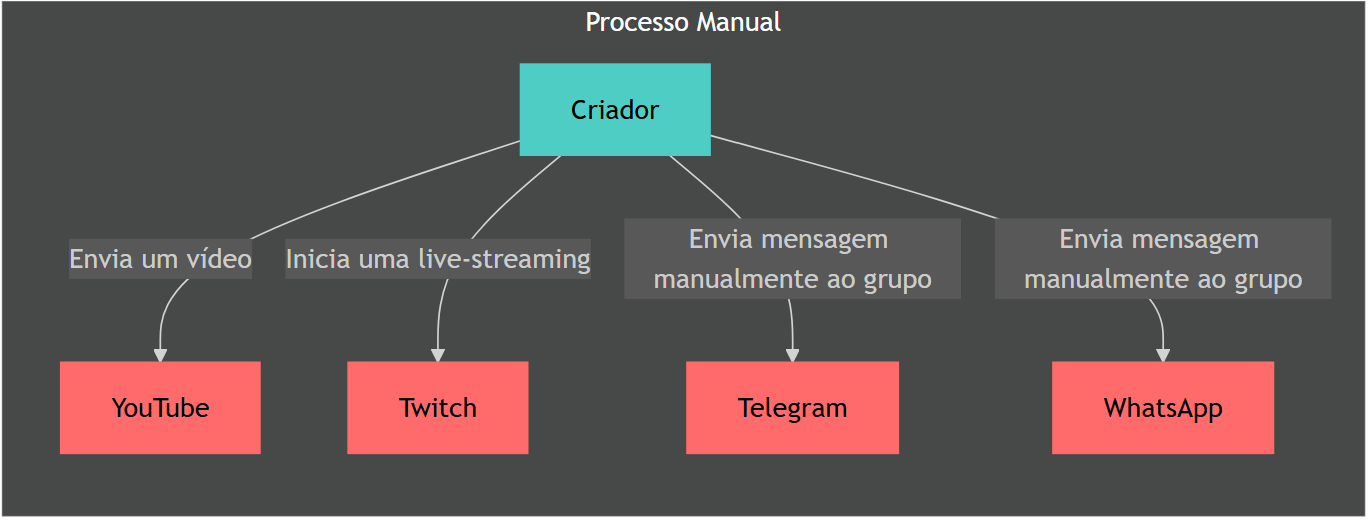
\includegraphics[width=1.0\linewidth]{img/processo manual.PNG}
    \label{fig:envio-manual}
\end{figure}

%##################  Imagem do processo de envio das notificações automatizado pelo sistema. Autoria própria
\begin{figure}[!ht]
    \centering
    \caption{
        Processo de Envio das Notificações Automatizado pelo Sistema.\\{\footnotesize\textbf{Fonte:} Autoria Própria.}
    }
    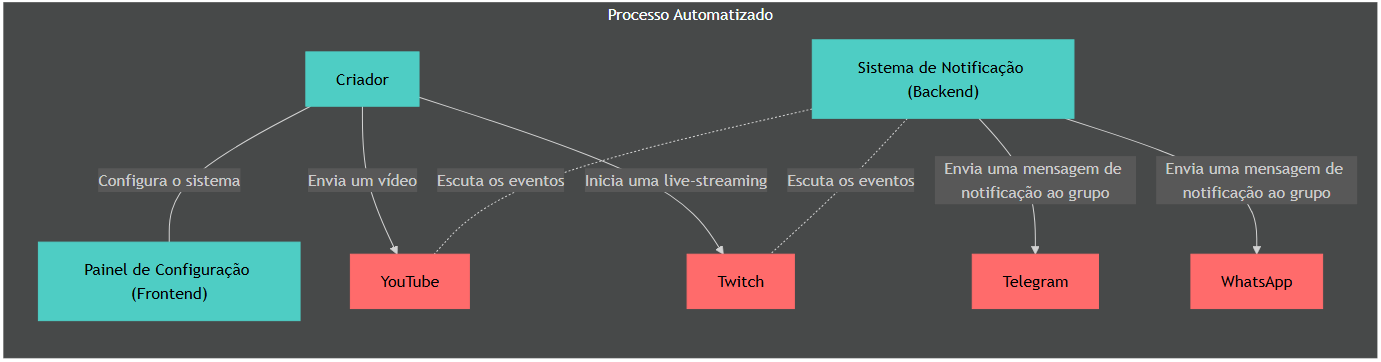
\includegraphics[width=1.0\textwidth]{img/processo automatizado.PNG}
    \label{fig:envio-automatizado}
\end{figure}

%##################  Imagem do Fluxo de Configuração da Aplicação pelo Painel. Autoria própria
\begin{figure}[!ht]
    \caption{
        Fluxo de Configuração da Aplicação pelo Painel.\\
        {\footnotesize\textbf{Fonte:} Autoria Própria.}
    }
    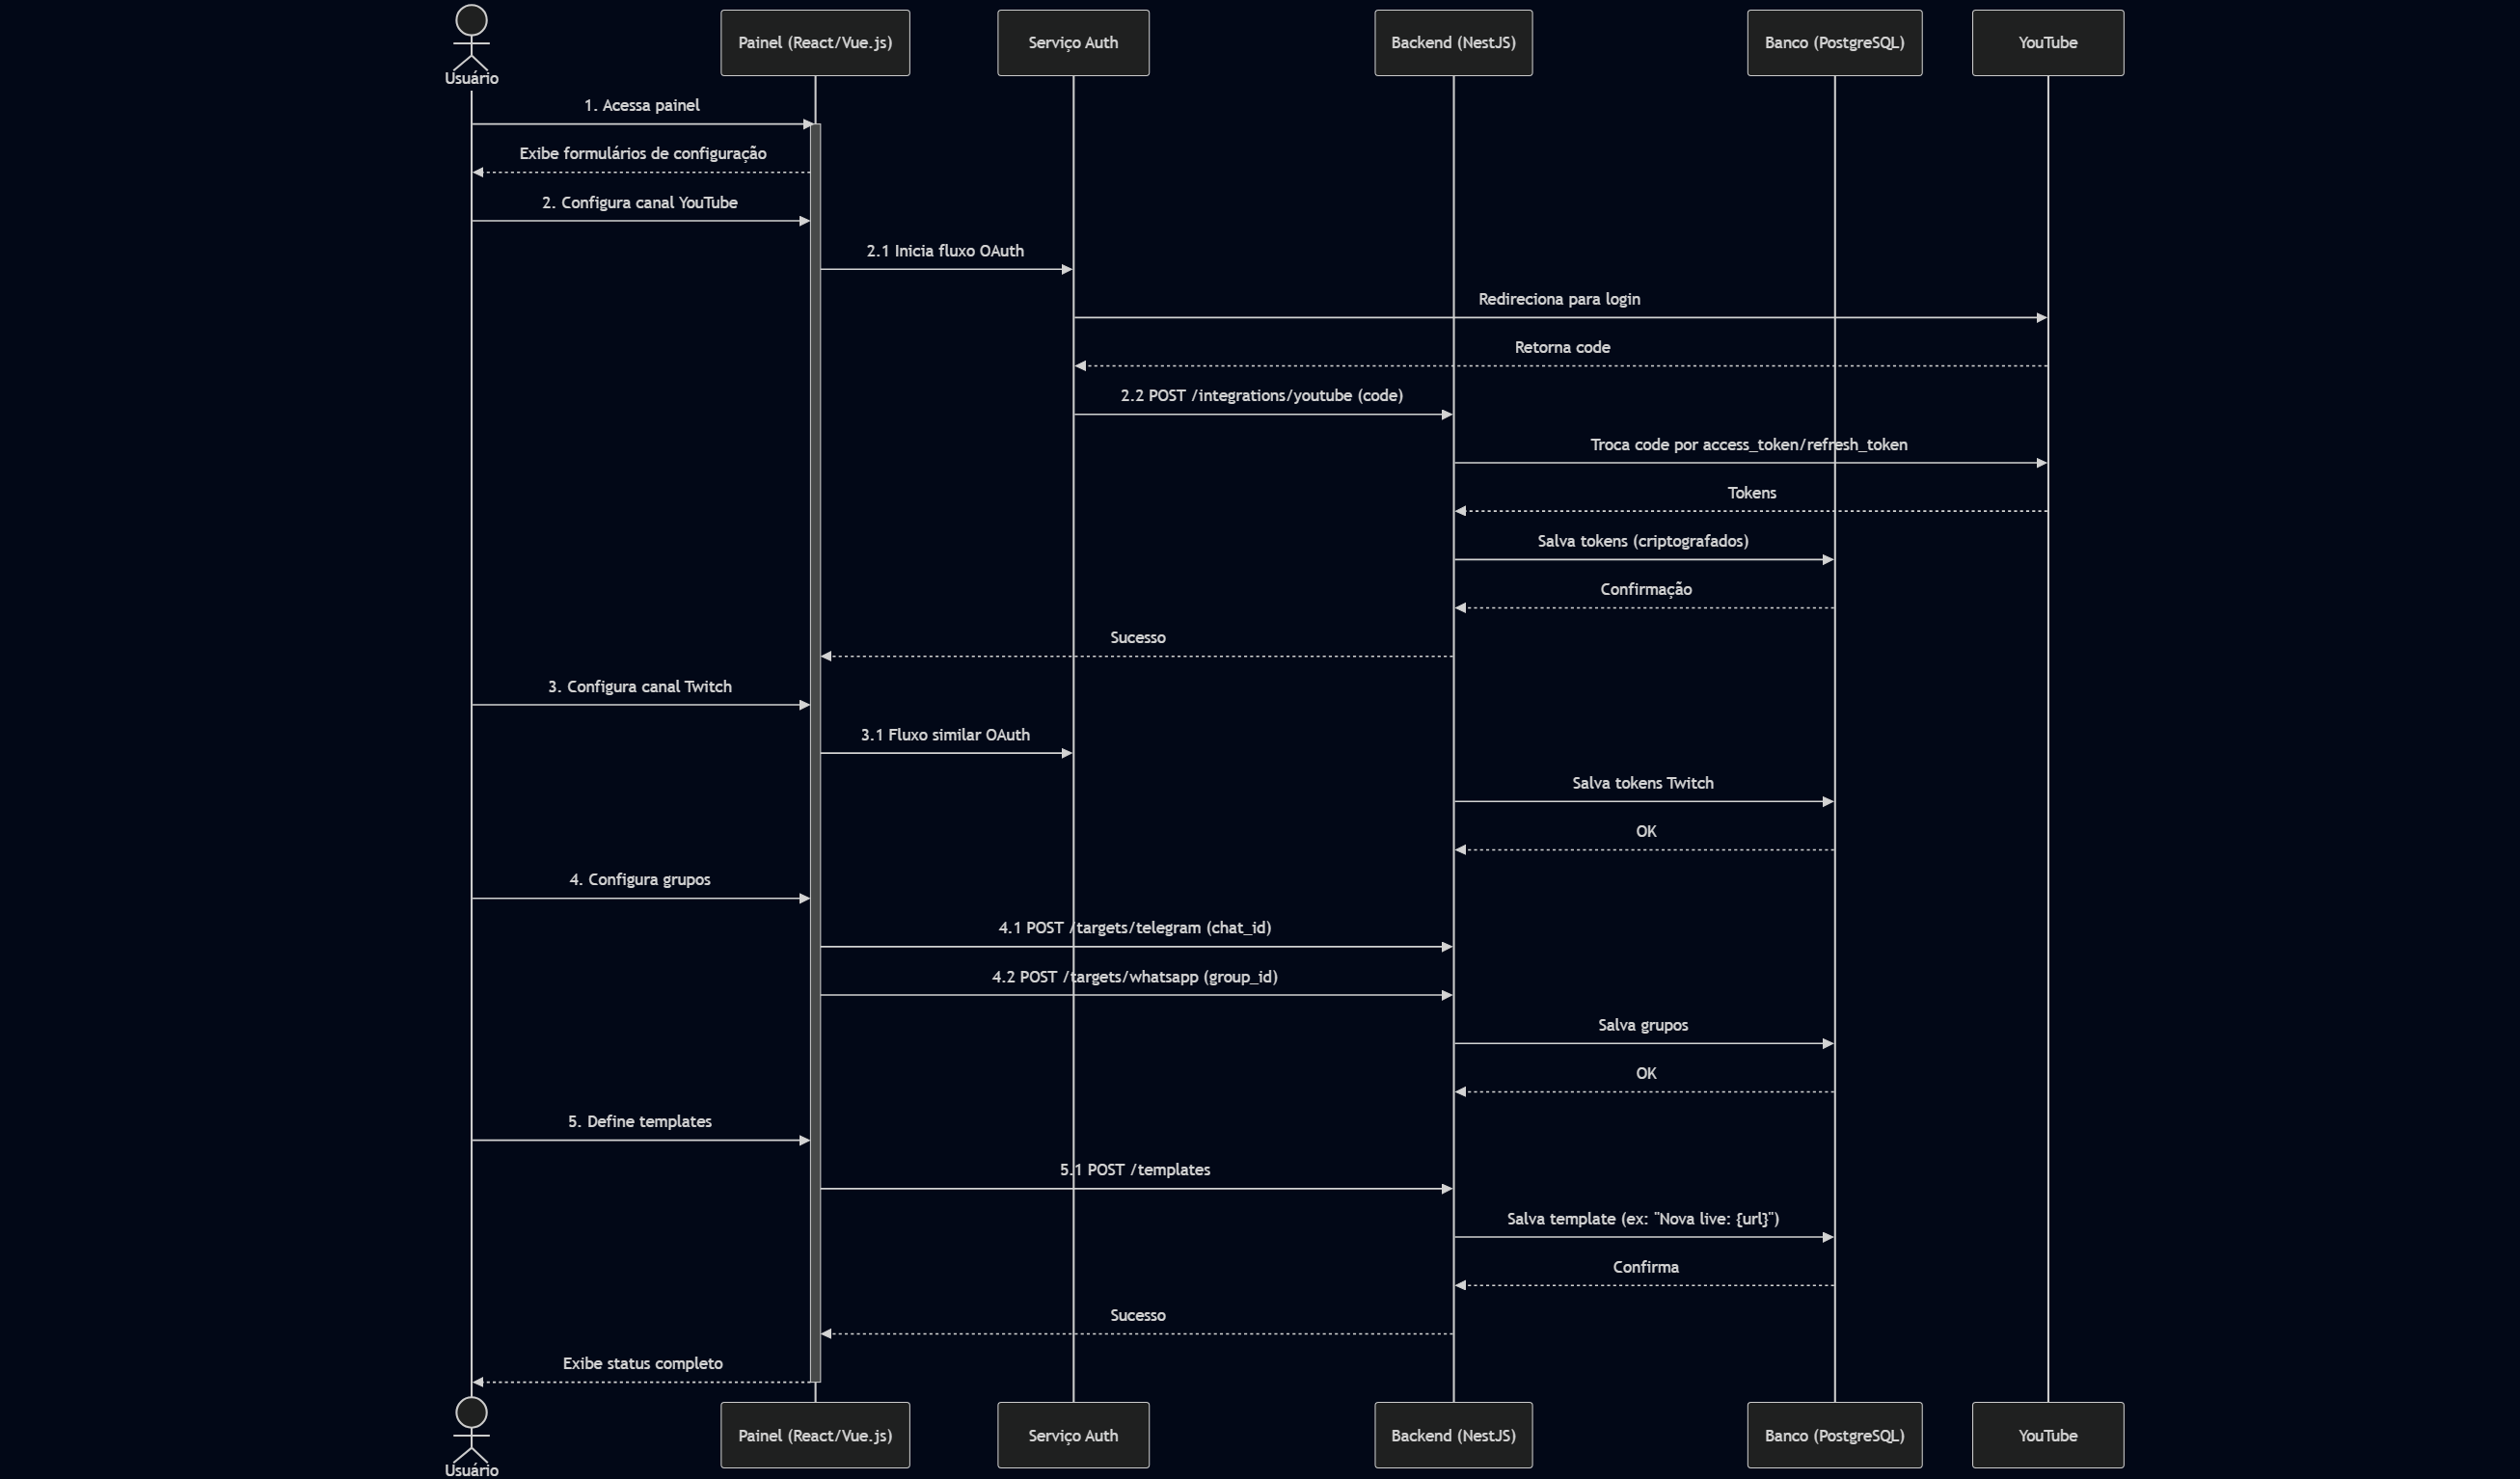
\includegraphics[width=1.0\textwidth]{img/Fluxo de Configuração da Aplicação pelo Painel.png}
    \label{fig:painel-configuracao}
\end{figure}

Do ponto de vista técnico, o projeto permite aprofundar conhecimentos em integração de sistemas via API, autenticação segura, comunicação assíncrona e arquitetura de sistemas Web escaláveis. Assim, este trabalho também contribui para formação pessoal como desenvolvedor, ao aplicar conhecimentos teóricos em um problema atual e concreto. A proposta pode ainda servir de base para melhorias ou ampliações futuras, como suporte a outras plataformas ou recursos avançados de análise de engajamento.
%-----------------------------------------------------------------------------------------


\section{REFERÊNCIAL TEÓRICO}
\label{sec:estadoarte}
% Estado da Arte--------------------------------------------------------------------------
% (máximo de 2 páginas)

Antes de detalhar os aspectos técnicos envolvidos na construção da solução proposta, é fundamental compreender o contexto sociocultural no qual ela se insere. Este trabalho parte da premissa de que tecnologias de automação e integração entre plataformas digitais não operam de forma isolada, mas sim dentro de um ecossistema interativo, dinâmico e orientado pelo comportamento de seus usuários. Assim, esta seção apresenta inicialmente as contribuições teóricas relacionadas à comunicação digital e ao engajamento em plataformas de \textit{streaming}, estabelecendo as motivações e necessidades que justificam a implementação de sistemas de notificação em tempo real. Em seguida, são exploradas as bases tecnológicas que viabilizam a proposta, incluindo protocolos de comunicação, APIs, arquitetura de \textit{software} e ferramentas utilizadas no desenvolvimento da solução.

\subsection{Bases Teóricas do Engajamento Digital}

%Nesta seção são abordados os principais conceitos e tecnologias que fundamentam o desenvolvimento da proposta, com foco em comunicação digital, integração via APIs, desenvolvimento \textit{Web} e automação de notificações em tempo real. O objetivo é evidenciar as bases técnicas e teóricas que sustentam a solução proposta, além de demonstrar que o problema investigado ainda apresenta lacunas que justificam novas abordagens.

A seguir, são apresentados os conceitos fundamentais relacionados ao comportamento e às motivações dos usuários em ambientes digitais. Aborda-se como fatores socioculturais influenciam o engajamento e a interação nas plataformas digitais, oferecendo o pano de fundo para o desenvolvimento das soluções propostas.

\subsubsection{Compreender a Gamificação na Plataforma Twitch.Tv: Aplicação da Teoria de Usos e Gratificações}

Em sua dissertação, Mariana da Silva Chilro caracteriza as plataformas de \textit{live streaming} como \textit{Social Live Streaming Services} (SLSSs), nas quais a comunicação ocorre em tempo real, favorecendo a interação imediata entre criadores e público \cite{daSilvaChilro2023}. Essa definição fundamenta a adoção de notificações em tempo real em sistemas destinados a monitorar canais no YouTube e na Twitch, garantindo que criadores sejam informados instantaneamente sobre atividades relevantes em suas transmissões.

% Em sua explanação sobre a Teoria dos Usos e Gratificações (TUG), Chilro retoma a definição de \cite{Katz&Blumler&Gurevitch1973} de que os indivíduos optam por consumir certos tipos de mídia, pois têm a expectativa de obter gratificações específicas como consequência de tais seleções. Essa teoria justifica a inclusão de notificações personalizadas, pois atende às necessidades cognitivas, afetivas e sociais dos usuários, aumentando a adesão ao sistema \cite{daSilvaChilro2023}.
% \par\vspace{0.75\baselineskip}

% %##################  Imagem com fluxo de Necessidade Cognitiva. Autoria própria
% \begin{figure}[htbp]
%     \centering
%     \caption{
%         \centering
%         Fluxo de Necessidade Cognitiva.\\
%         {\footnotesize\textbf{Fonte:} Autoria Própria.}
%     }
%     
\includegraphics[width=0.9\textwidth]{img/necessidade cognitiva.PNG}
%     \label{fig:necessidade-cognitiva}
% \end{figure}

% \par\vspace{0.75\baselineskip}
Por fim, o conceito de \textit{consumer engagement} é apresentado como multidimensional — envolvendo aspectos cognitivos, emocionais e comportamentais — e associado ao aumento da retenção e do suporte financeiro ao criador \cite{daSilvaChilro2023}. Essa perspectiva serve de base para justificar a necessidade de notificações ágeis e personalizadas, capazes de manter a comunidade ativa e mutuamente engajada.

\subsubsection{Fatores de Sucesso para Canais de \textit{Live Streaming} de Jogos Online na Percepção dos Usuários Brasileiros da Twitch.tv}

Em seu trabalho \cite{matsumoto2019} destaca o crescimento exponencial das transmissões ao vivo de jogos eletrônicos e a consequente consolidação da Twitch como principal plataforma desse segmento. Ele aponta que, em 2018, os usuários brasileiros assistiram a impressionantes 9,36 bilhões de horas de conteúdo na Twitch, indicando não apenas o alcance da plataforma, mas também a importância da interatividade proporcionada pelo chat em tempo real e pela formação de comunidades virtuais em torno dos \textit{streamers}.

Além disso, Matsumoto evidencia que a interação via chat em tempo real favorece a criação e consolidação de comunidades virtuais em torno dos \textit{streamers}, promovendo um senso de pertencimento entre os espectadores. Além disso, o autor enfatiza que mecanismos de engajamento, como o envio de alertas de início de transmissão (notificações) aos seguidores, são reconhecidos como funcionalidades cruciais para manter a audiência informada e incentivar o consumo de conteúdo ao vivo, embora o estudo não apresente dados quantitativos sobre sua eficácia \cite{matsumoto2019}.
\
%Nova organização
%%%%%%%%%%%%%%%%%%%%%%%%%%%%%%%%%%%%%%%%%%%%%%%%%%%%%%%%%%%%%%
% \subsection{Comunicação e Engajamento em Plataformas Digitais}
% \begin{itemize}
%     \item A importância da comunicação instantânea para criadores de conteúdo. \cite[p. 2]{matsumoto2019}
%     \item O papel das notificações na retenção de audiência e engajamento de comunidades online. \cite[p. 24]{daSilvaChilro2023}
%     \item Estudos sobre comportamento de audiência em transmissões ao vivo e canais de vídeo. \cite[p. 102]{daSilvaMachado&Dutra2022}
% \end{itemize}

\subsection{Bases Técnicas e Tecnológicas}

% A seguir são apresentados os conceitos fundamentais sobre APIs, a forma como permitem a integração entre diferentes serviços e um trabalho semelhante ao que está sendo desenvolvido neste TCC.

A seguir são apresentados conceitos de API REST, incluindo padrões de design, estratégias de autenticação e análise comparativa entre APIs públicas e privadas. Além disso, serão apresentados estudos de caso análogos ao projeto central desta pesquisa, demonstrando aplicações práticas dos conceitos discutidos

\subsubsection{WhatsDine: Solução para o \textit{Delivery} Integrada ao WhatsApp}

O trabalho de \cite{abreu2023} apresenta o WhatsDine, uma plataforma de \textit{delivery} que explora o amplo alcance do WhatsApp para gerenciar pedidos entre clientes e restaurantes de pequeno e médio porte. Além disso, mostra como aproveitar o WhatsApp como canal de disparo de alertas em tempo real. Para isso, Abreu utiliza o \textit{whatsapp-web.js} — uma biblioteca que executa em \textit{background} uma instância real do WhatsApp Web, expondo uma API local capaz de enviar e receber mensagens sem depender de serviços pagos ou da Whatsapp Cloud API oficial. Com essa integração, o sistema automatiza o envio de mensagens em cada etapa do fluxo de pedidos — desde a escolha de itens até a confirmação de pagamento — usando funcionalidades nativas de chat do WhatsApp para manter todas as interações em um único canal.

\subsubsection{Criação de APIs REST para Gestão de \textit{Bots} Inteligentes no WhatsApp Utilizando os Modelos Whisper e Chat GPT para Aplicação no Sistema Doumi}

O trabalho de \cite{dias2024} apresenta uma arquitetura modular para o envio e gerenciamento de notificações via WhatsApp, fundamentada na emissão de \textit{webhooks} que sincronizam eventos em tempo real entre as APIs. Sempre que uma mensagem é recebida pelo \textit{whatsapp-web.js} e chega ao fim da fila de processamento, é disparado um \textit{webhook} para a API de \textit{back‑end}, que executa a lógica necessária para gerar e enviar a resposta adequada ao usuário . 

Para garantir a confiabilidade e o desempenho em cenários de alta demanda, as mensagens são gerenciadas por meio de uma fila assíncrona, onde cada evento emitido pelo \textit{Whatsapp-web.js} é enfileirado e aguarda um intervalo de 10 segundos antes de ser enviado. Caso novas mensagens do mesmo cliente cheguem durante esse período, elas são concatenadas e despachadas em uma única requisição ao \textit{webhook} do \textit{back‑end}, otimizando o uso de recursos e evitando chamadas redundantes \cite{dias2024}. 

A comunicação entre as APIs WhatsApp e \textit{back‑end} ocorre via \textit{endpoints} RESTful e \textit{webhooks}, promovendo trocas de informações seguras e consistentes. Esse fluxo permite tratar erros, controlar \textit{rate limits} e manter os estados de conexão sincronizados, assegurando escalabilidade e facilidade de manutenção do sistema como um todo \cite{dias2024}.

\subsubsection{Desenvolvimento de APIs Baseadas em REST para Integração e
Construções de Aplicações.}

\cite{campos2013} define API como uma interface que permite a comunicação entre aplicações computacionais, funcionando como um contrato técnico e de negócio por meio de documentação, regras de uso, limites de consumo e políticas de marca. Essa definição ressalta que a API deve garantir interoperabilidade, previsibilidade e governança nas integrações entre diferentes aplicações.

Para o design de APIs RESTful, Campos detalha a série de decisões que compõem uma interface alinhada ao estilo arquitetural REST. Ele enfatiza quatro métodos HTTP principais — \textit{GET}, \textit{POST}, \textit{PUT} e \textit{DELETE} — correspondentes às operações CRUD. Ele destaca o uso de JSON — exemplificado na Figura \ref{fig:json} — como formato predominante para serialização de dados, a adoção de URIs claras e semânticas conforme a definido pela RFC 3986, e a importância de cabeçalhos “\textit{Accept}”, “\textit{Content-Language}”, “\textit{Last-Modified}” e “\textit{Content-Type}” — exemplificados nas Figuras \ref{fig:accept} e \ref{fig:content-type-language} — para negociação de conteúdo \cite{campos2013}.

%##################  Imagem com exemplo do uso de Accept. Adaptado do livro RESTful \textit{Web} Services Cookbook de Subbu Allamaraju, 2010
\begin{figure}[!ht]
    \centering
    \caption{
        Exemplo do uso de \textit{Accept}.\\
        {\footnotesize\textbf{Fonte:} Autoria Própria.}
    }
    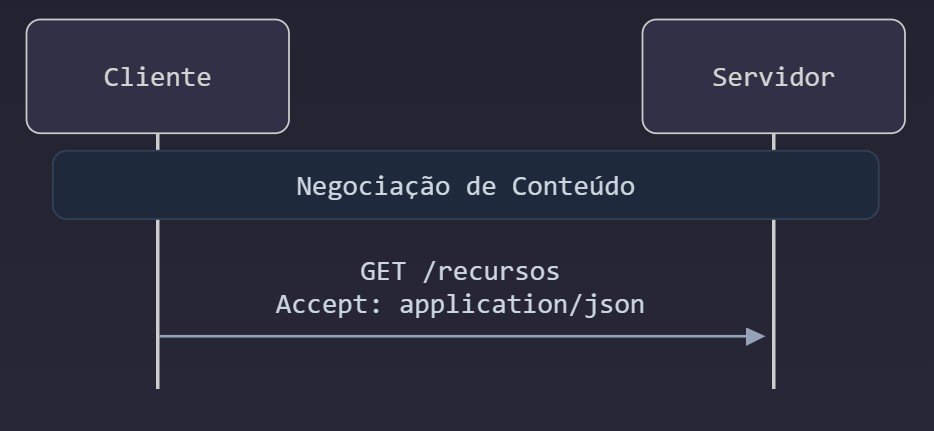
\includegraphics[width=0.8\textwidth]{img/Exemplo do uso de Accept.jpg}
    \label{fig:accept}
\end{figure}

%##################  Imagem com exemplo do uso de Content-Type, Content-Language e Last-Modified. Adaptado do livro RESTful \textit{Web} Services Cookbook de Subbu Allamaraju, 2010
\begin{figure}[H]
    \centering     
    \caption{
        Exemplo do uso de \textit{Content-Type}, \textit{Content-Language} e \textit{Last-Modified}.\\
        {\footnotesize\textbf{Fonte:} Adaptado de \citeonline{allamaraju2010}.}
    }
    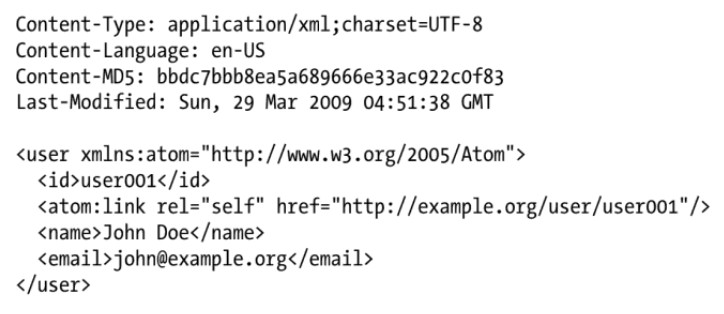
\includegraphics[width=0.8\textwidth]{img/Exemplo do uso de Content-Type Content-Language Last-Modified.jpg}
    \label{fig:content-type-language}
\end{figure}

%##################  Imagem com exemplo de JSON. Adaptado do trabalho do Campos, 2013
\begin{figure}[H]
    \centering     
    \caption{
        Exemplo do uso de JSON.\\
        {\footnotesize\textbf{Fonte:} Adaptado de \citeonline{campos2013}.}
    }
    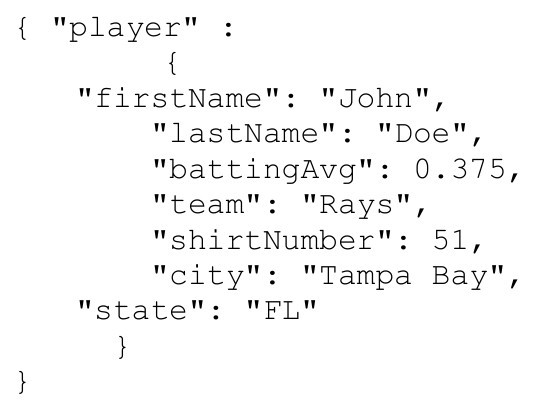
\includegraphics[width=0.5\textwidth]{img/Exemplo de JSON - Campos.jpg}
    \label{fig:json}
\end{figure}

No que tange à autenticação, Campos aborda desde o emprego simples de \textit{API Keys} até a adoção do \textit{framework} OAuth2 para cenários que exigem emissão de \textit{tokens} e escopos mais granulares. Essa diversidade de mecanismos permite ajustar o nível de segurança conforme o contexto de uso da API \cite{campos2013}. 

Entre as boas práticas para design de APIs REST, o autor destaca: uso de URIs sem verbos, padronizadas em plural e minúsculas; versionamento de \textit{endpoints} via caminho (e.g. “/v1/recursos”); paginação usando os parâmetros “\textit{limit}” e “\textit{offset}” — exemplificados na Figura \ref{fig:offset-limit} — e tratamento consistente de erros com códigos HTTP adequados (405, 404, 500 etc.) \cite{campos2013}.
\par\vspace{0.75\baselineskip}

%##################  Imagem com exemplo de uso de offset e limit. Adaptado do trabalho do Campos, 2013
\begin{figure}[H]
    \centering     
    \caption{
        Exemplo de uso de \textit{offset} e \textit{limit}.\\
        {\footnotesize\textbf{Fonte:} Retirado de \citeonline{campos2013}.}
    }
    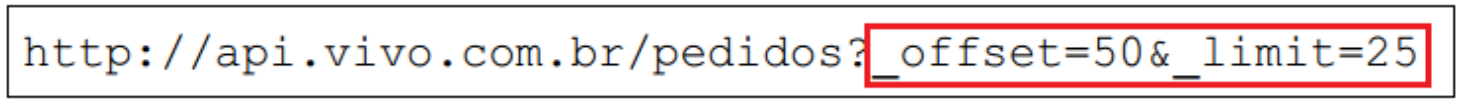
\includegraphics[width=0.9\textwidth]{img/Exemplo do uso de offset e limits.PNG}
    \label{fig:offset-limit}
\end{figure}

\par\vspace{0.75\baselineskip}
Ao discutir APIs públicas, Campos destaca que permitem a rápida disponibilização de funcionalidades já consolidadas, ampliam o alcance da marca ao fomentar a criação de ecossistemas de terceiros e estimulam a inovação por meio dessas comunidades externas. Essas características tornam o modelo particularmente eficiente para organizações que desejam promover parcerias e acelerar o desenvolvimento de novos produtos, sem retrabalho no reaproveitamento de recursos já existentes \cite{campos2013}.

Já no contexto das APIs privadas, o autor enfatiza o acesso restrito a desenvolvedores ou equipes internas, o que reforça a segurança através de mecanismos como SSL, HTTP \textit{Basic} ou OAuth2. Além disso, ressalta a redução de custos de manutenção e a agilidade na integração com processos internos, resultando em entregas de serviços mais rápidas e controladas \cite{campos2013}.

% \subsection{Integração entre Plataformas: APIs e Protocolos de Comunicação}

% \subsection{Conceitos de API e Integração de Sistemas}
% \begin{itemize}
%     \item Definição de API (Interface de Programação de Aplicações).
%     \item Estrutura de APIs \textit{RESTful}: métodos HTTP, autenticação, boas práticas.
%     \item Vantagens e limitações das APIs públicas no desenvolvimento de sistemas.
% \end{itemize}

\subsection{APIs}

%As principais APIs utilizadas no desenvolvimento da proposta são:

A integração entre sistemas modernos frequentemente depende da comunicação com serviços externos por meio de APIs. No contexto deste trabalho, são exploradas diversas APIs voltadas à coleta, processamento e envio de informações em tempo real, possibilitando a construção de soluções automatizadas e conectadas. Estas interfaces permitem o acesso a plataformas amplamente utilizadas, como YouTube, Twitch, Telegram, WhatsApp, viabilizando funcionalidades como notificações instantâneas, monitoramento de eventos, e interação com usuários por meio de canais digitais diversos.

A seguir, apresentam-se as principais APIs utilizadas no projeto, com uma breve descrição de suas funcionalidades e relevância para os objetivos propostos:
\par\vspace{0.5\baselineskip}

%\footnote{Disponível em: \url{https://developers.google.com/youtube/v3?hl=pt-br}}
\begin{enumerate}
    \item \textbf{YouTube Data API}\footnote{Disponível em: \url{https://developers.google.com/youtube/v3}. Acessado em: 06/06/2025.} - Oferece acesso a um vasto conjunto de recursos relacionados a vídeos, canais e \textit{playlists} na plataforma do YouTube. Ela possibilita, por exemplo, a realização de buscas avançadas, acesso a estatísticas e gerenciamento de conteúdo. Em propostas que envolvem a disseminação de notificações ou a coleta de dados multimídia, essa API desempenha um papel fundamental, tornando possível a automação de processos e o monitoramento contínuo das atualizações em canais de interesse.
    \par\vspace{0.25\baselineskip}
    
    \item \textbf{Twitch API}\footnote{Disponível em: \url{https://dev.twitch.tv/docs/api/}. Acessado em: 06/06/2025.} - É a interface oficial da plataforma Twitch para acesso a dados e eventos relacionados a transmissões ao vivo. Por meio dela, é possível obter informações sobre canais, \textit{streams}, seguidores e eventos de interação do público. A API utiliza o protocolo OAuth2 para autenticação garantindo uma comunicação segura e eficiente. Esses recursos são essenciais para aplicações que precisam integrar notificações e monitorar eventos em tempo real no ambiente dos games e transmissões.
    \par\vspace{0.25\baselineskip}
    
    \item \textbf{Telegram Bot API}\footnote{Disponível em: \url{https://core.telegram.org/api}. Acessado em: 06/06/2025.} - Permite a integração simplificada de \textit{bots}—contas especiais que não exigem número de telefone cadastrados no servidor. Utilizando uma interface HTTPS, o serviço cuida automaticamente da criptografia (MTProto), possibilitando o envio e recebimento de mensagens, comandos interativos e o gerenciamento seguro de \textit{chats} e grupos.
    \par\vspace{0.25\baselineskip}
    
    \item \textbf{\textit{Whatsapp-web.js}}\footnote{Disponível em: \url{https://wwebjs.dev/}. Acessado em: 06/06/2025.} - Apesar de não ser uma API oficial do WhatsApp, o \textit{whatsapp-web.js} é uma biblioteca que permite a integração com o WhatsApp Web. Ela possibilita a criação de \textit{scripts} que automatizam o envio e recebimento de mensagens, além de oferecer métodos para a manipulação de chats e contatos. Essa ferramenta é especialmente útil para implementações que visam a comunicação automatizada, permitindo a criação de fluxos personalizados de interação sem depender das limitações das APIs oficiais.
    \par\vspace{0.25\baselineskip}  
    
    % \item \textbf{Twilio API}\footnote{Disponível em: \url{https://www.twilio.com/docs/whatsapp}. Acessado em: 06/06/2025.} - É uma interface RESTful que, usando seu \textit{Account SID} e \textit{Auth Token}, permite enviar e receber mensagens pelo WhatsApp. Você precisa de um número habilitado (em modo \textit{Sandbox} para testes ou produção com número verificado). Ela suporta texto, mídia (imagens, áudio, vídeo, documentos) e \textit{templates} aprovados pelo WhatsApp Business, além de \textit{webhooks} para rastrear entregas, leituras e respostas. Há bibliotecas oficiais (Node.js, Python, Java, PHP etc.) e um console web, facilitando o envio de notificações, confirmações e o gerenciamento de conversas via WhatsApp.
\end{enumerate}

%%%%%%%%%%%%%%%%%%%%%%%%%%%%%%%%%%%%%%%%%%%%%%%%%%%%%%%%%%%%%%

% Uma vez formulado o problema a ser atacado, é preciso se inteirar do que já foi feito, dito e discutido sobre ele. Isso se chama "estado da arte". Pode ser que a dúvida, que está motivando a pesquisa, já tenha sido respondida de alguma maneira por alguém. Por isso, é preciso aprofundar o conhecimento sobre a questão, antes de dar prosseguimento ao projeto.

% Essa etapa também recebe o nome de revisão bibliográfica, quando são estudados os trabalhos que se situam na circunvizinhança do problema, trabalhos que versam sobre problemas similares.

% Vê-se aí por que a revisão bibliográfica é importante. De um lado, ela deve comprovar que o pesquisador não está querendo realizar algo que já foi feito, de outro lado, ela ajuda a encaminhar o passo seguinte da pesquisa, a justificativa, quer dizer, a argumentação sobre a relevância do trabalho.

% Para a proposta de TCC deve ser descrito, de maneira breve, alguns (sugestão de 2 (dois) a 3 (três)) trabalhos correlatos, converse com seu orientador para citar os mais relevantes do tema abordado. Pode ser seguido a seguinte sugestão de parágrafos/tópicos:

% P1. Descrição do trabalho 1

% P2. Descrição do trabalho 2

% P3. Descrição do trabalho 3

% P4. Discussão dos trabalhos mencionados destacando porque eles são importantes para o trabalho proposto.

% Para utilização de citações atente ao tipo de citação que se deseja usar. As citações são classificadas em indeireta e direta, podem ser longas ou curtas.

% Uma citação indireta é a transcrição, com suas próprias palavras, das idéias de um autor, mantendo-se o sentido original. A citação indireta é a maneira que o pesquisador tem de ler, compreender e gerar conhecimento a partir do conhecimento de outros autores. Quanto à chamada da referência, ela pode ser feita de duas maneiras distintas, conforme o nome do(s) autor(es) façam parte do seu texto ou não. Exemplo de chamada fazendo parte do texto:\\
% \\Enquanto \citeonline{Maturana2003} defendem uma epistemologia baseada na biologia. Para os autores, é necessário rever \ldots.\\

% A chamada de referência foi feita com o comando \verb|\citeonline{chave}|, que produzirá a formatação correta.

% A segunda forma de fazer uma chamada de referência deve ser utilizada quando se quer evitar uma interrupção na sequência do texto, o que poderia, eventualmente, prejudicar a leitura. Assim, a citação é feita e imediatamente após a obra referenciada deve ser colocada entre parênteses. Porém, neste caso específico, o nome do autor deve vir em caixa alta, seguido do ano da publicação. Exemplo de chamada não fazendo parte do texto:\\
% \\Há defensores da epistemologia baseada na biologia que argumentam em favor da necessidade de \ldots \cite{Maturana2003}.\\

% Nesse caso a chamada de referência deve ser feita com o comando \verb|\cite{chave}|, que produzirá a formatação correta.

% Uma citação direta é a transcrição ou cópia de um parágrafo, de uma frase, de parte dela ou de uma expressão, usando exatamente as mesmas palavras adotadas pelo autor do trabalho consultado.

% Quanto à chamada da referência, ela pode ser feita de qualquer das duas maneiras, assim como nas nas citações indiretas, conforme o nome do(s) autor(es) façam parte do texto ou não. Há duas maneiras distintas de se fazer uma citação direta, conforme o trecho citado seja longo ou curto.

% Quando o trecho citado é longo (4 ou mais linhas) deve-se usar um parágrafo específico para a citação, na forma de um texto recuado (4 cm da margem esquerda), com tamanho de letra menor e espaçamento entrelinhas simples. Exemplo de citação longa:
% \\\begin{citacao}
% Desse modo, opera-se uma ruptura decisiva entre a reflexividade filosófica, isto é a possibilidade do sujeito de pensar e de refletir, e a objetividade científica. Encontramo-nos num ponto em que o conhecimento científico está sem consciência. Sem consciência moral, sem consciência reflexiva e também subjetiva. Cada vez mais o desenvolvimento extraordinário do conhecimento científico vai tornar menos praticável a própria possibilidade de reflexão do sujeito sobre a sua pesquisa \cite[p.~28]{Silva2000}.
% \end{citacao}

% Para fazer a citação longa deve-se utilizar os seguintes comandos:
% \begin{verbatim}
% \begin{citacao}
% <texto da citacao>
% \end{citacao}
% \end{verbatim}

% No exemplo acima, para a chamada da referência o comando \verb|\cite[p.~28]{Silva2000}| foi utilizado, visto que os nomes dos autores não são parte do trecho citado. É necessário também indicar o número da página da obra citada que contém o trecho citado.

% Quando o trecho citado é curto (3 ou menos linhas) ele deve inserido diretamente no texto entre aspas. Exemplos de citação curta:\\
% \\A epistemologia baseada na biologia parte do princípio de que "assumo que não posso fazer referência a entidades independentes de mim para construir meu explicar" \cite[p.~35]{Maturana2003}.\\
% \\A epistemologia baseada na biologia de \citeonline[p.~35]{Maturana2003} parte do princípio de que "assumo que não posso fazer referência a entidades independentes de mim para construir meu explicar".\\

% Outros exemplos de comandos para as chamadas de referências e o resultado produzido por estes são:\\
% \\\citeonline{Maturana2003} \ \ \  \verb|\citeonline{Maturana2003}|\\
% \citeonline{Barbosa2004} \ \ \   \verb|\citeonline{Barbosa2004}|\\
% \cite[p.~28]{Silva2000} \ \ \  \verb|\cite[p.~28]{Silva2000}|\\
% \citeonline[p.~33]{Silva2000} \ \ \   \verb|\citeonline[p.~33]{v}|\\
% \cite[p.~35]{Maturana2003} \ \ \   \verb|\cite[p.~35]{Maturana2003}|\\
% \citeonline[p.~35]{Maturana2003} \ \ \   \verb|\citeonline[p.~35]{Maturana2003}|\\
% \cite{Barbosa2004,Maturana2003} \ \ \   \verb|\cite{Barbosa2004,Maturana2003}|\\

% Em relação as referências, a bibliografia é feita no padrão \textsc{Bib}\TeX{}. As referências são colocadas em um arquivo separado. Neste template as referências são armazenadas no arquivo "base-referencias.bib".

% Existem diversas categorias documentos e materiais componentes da bibliografia. A classe abn\TeX{} define as seguintes categorias (entradas):

% \begin{verbatim}
% @book
% @inbook
% @article
% @phdthesis
% @mastersthesis
% @monography
% @techreport
% @manual
% @proceedings
% @inproceedings
% @journalpart
% @booklet
% @patent
% @unpublished
% @misc
% \end{verbatim}

% Cada categoria (entrada) é formatada pelo pacote \citeonline{abnTeX22014d} de uma forma específica. Para maiores detalhes, refira-se a \citeonline{abnTeX22014d}, \citeonline{abnTeX22014b}, \citeonline{abnTeX22014c}.

% %-----------------------------------------------------------------------------------------

% % \subsection{DIFERENCIAL TECNOLÓGICO}
% % \label{sec:diferencial}
% % 
% % Diferencial Tecnológico-----------------------------------------------------------------
% % (máximo de ½ página)
% % O diferencial teórico é uma complementação do tópico discussão da seção estado da arte, onde será evidenciado qual o diferencial do trabalho perante os demais correlatos já existentes. Deve-se destacar os seguintes itens:

% % Diferencial do trabalho proposto perante produtos concorrentes ou semelhantes;

% % Vantagens que os possíveis usuários terão ao usar o trabalho a ser desenvolvido;

% % Destacar inovação tecnológica, por exemplo, uso de novas tecnologias e vantagens;

% % (substitua este texto pelo diferencial tecnológico do trabalho)

%-----------------------------------------------------------------------------------------

\section{MATERIAIS E MÉTODOS} % Escolher o nome mais adequado ao trabalho
\label{sec:metodologia}
% Esta seção descreve os recursos necessários e os procedimentos adotados para o desenvolvimento, implantação e validação do sistema proposto. Ao detalhar cada componente de hardware, \textit{software} e as abordagens metodológicas, busca-se garantir a reprodução dos experimentos e a clareza quanto às etapas envolvidas no projeto.

Esta seção apresenta os recursos utilizados na implementação da proposta, incluindo os itens de hardware e ferramentas de desenvolvimento que compõem a base tecnológica do sistema. A seleção desses materiais teve como objetivo garantir um ambiente de desenvolvimento consistente, capaz de proporcionar testes reais, integração com serviços externos e desempenho confiável em aplicações modernas. 

A organização dos conteúdos está estruturada de forma a refletir os principais componentes da arquitetura da aplicação: (i) as linguagens e o ambiente de execução utilizados no desenvolvimento da aplicação principal; (ii) os mecanismos de processamento assíncrono e gerenciamento de filas, essenciais para garantir o desempenho paralelo e em tempo real de tarefas; e (iii) as soluções de armazenamento de dados, voltadas para a persistência, consulta e integridade das informações. Também são descritas (iv) as ferramentas de teste e qualidade de código, além (v) das tecnologias utilizadas na construção da interface do usuário.

\subsection{Materiais}
    A seguir, apresenta-se a lista de itens de hardware, ferramentas de desenvolvimento que serão utilizadas neste trabalho. Esses recursos foram selecionados para proporcionar um ambiente de desenvolvimento consistente e capaz de suportar testes reais de notificação e integração com serviços externos.
    \par\vspace{0.5\baselineskip}
    
    \begin{enumerate}
        \item \textbf{Hardware:}  
        \begin{itemize}
            \item Computador pessoal com pelo menos 16 GB de RAM, processador \textit{quad-core} e SSD (Windows 10/11).  
            \par\vspace{0.25\baselineskip}

            \item Smartphone Android para testes de recebimento de notificações.  
            \par\vspace{0.75\baselineskip}
        \end{itemize}

        \item \textbf{Linguagens e Ambiente de Desenvolvim\textit{}ento:}  
        \begin{itemize}
            \item \textbf{TypeScript}\footnote{Disponível em: \url{https://www.typescriptlang.org/}. Acessado em: 06/06/2025.}: 
                O TypeScript é uma linguagem de programação construída como um \textit{superset} do JavaScript, que adiciona tipagem estática e recursos avançados de orientação a objetos. Essa tipagem robusta contribui para a redução de erros comuns em tempo de compilação, facilitando a manutenção e a escalabilidade do código. No contexto do desenvolvimento moderno, TypeScript tem se destacado por proporcionar uma base sólida para a construção de aplicações complexas e de larga escala. %\cite{typescript}
            \par\vspace{0.25\baselineskip}

            \item \textbf{Node.js}\footnote{Disponível em: \url{https://nodejs.org/}. Acessado em: 06/06/2025.}: 
                O Node.js é um ambiente de execução de JavaScript baseado no motor V8, que se caracteriza por seu modelo assíncrono e orientado a eventos. Essa abordagem permite a criação de aplicações altamente performáticas e escaláveis, especialmente em operações I/O intensivas, como conexões em tempo real e processamento paralelo de tarefas. A popularidade do Node.js também se deve à sua rica comunidade e ao ecossistema de bibliotecas, o que facilita a integração com diversas tecnologias e plataformas. %\cite{nodejs}
            \par\vspace{0.25\baselineskip}

            \item \textbf{NestJS}\footnote{Disponível em: \url{https://nestjs.com/}. Acessado em: 06/06/2025.}: 
                O NestJS é um \textit{framework} progressivo para Node.js construído com TypeScript que adota padrões de arquitetura modular e injeção de dependências. Baseado em Express, oferece suporte nativo a microserviços, WebSockets e GraphQL, além de um CLI para geração de código. Sua estrutura organizada e tipagem completa ajudam a criar aplicações escaláveis, testáveis e de fácil manutenção. %\cite{nestjs}
            \par\vspace{0.25\baselineskip}
            
            \item \textbf{Visual Studio Code (VSCode)}\footnote{Disponível em: \url{https://code.visualstudio.com/}. Acessado em: 06/06/2025.}:
                O VSCode é um editor de código‐fonte leve e gratuito desenvolvido pela Microsoft. Compatível com diversas linguagens de programação, ele oferece recursos como destaque de sintaxe, autocompletar inteligente, depuração integrada e controle de versão com Github. Sua grande variedade de extensões permite personalizar o ambiente de desenvolvimento de forma simples e eficiente.
            \par\vspace{0.25\baselineskip}

            \item \textbf{Windows Subsystem for Linux (WSL) 2}\footnote{Disponível em: \url{https://learn.microsoft.com/pt-br/windows/wsl/}. Acessado em: 06/06/2025.}: 
                O WSL2 é uma ferramenta da Microsoft que permite rodar distribuições Linux diretamente no Windows, com melhor desempenho e compatibilidade em relação à versão anterior. Utiliza um kernel Linux real e oferece integração entre os sistemas de arquivos do Windows e do Linux, facilitando o desenvolvimento de aplicações em ambiente Unix sem sair do Windows. %\cite{wsl2}
            \par\vspace{0.25\baselineskip}

            \item \textbf{Docker}\footnote{Disponível em: \url{https://www.docker.com/}. Acessado em: 07/06/2025.}: 
                O Docker é uma plataforma de containerização que empacota aplicações e suas dependências em ambientes isolados chamados \textit{containers}. Isso garante portabilidade entre diferentes sistemas e facilita o desenvolvimento, testes e \textit{deploy} contínuo. Com imagens leves e repositórios como o Docker Hub, simplifica a escalabilidade e a gestão de serviços em ambientes locais e na nuvem. %\cite{docker}
             \par\vspace{0.25\baselineskip}

            % \item \textbf{Git}\footnote{Disponível em: \url{https://git-scm.com/doc}. Acessado em: 06/06/2025.}: 
            %     O Git é um sistema de controle de versão distribuído \textit{open-source} projetado para gerenciar eficientemente projetos de qualquer escala. Seu modelo descentralizado permite que desenvolvedores trabalhem \textit{offline} e colaborem através de operações como \textit{commit}, \textit{branch} e \textit{merge}, garantindo rastreabilidade completa das alterações no código-fonte. A robustez na manipulação de histórico e resolução de conflitos o torna padrão na indústria para coordenação de trabalho em equipe.
            % \par\vspace{0.25\baselineskip}
            
            \item \textbf{Github}\footnote{Disponível em: \url{https://docs.github.com/pt}. Acessado em: 06/06/2025.}: 
                O GitHub é uma plataforma de hospedagem e colaboração baseada em Git para desenvolvimento de \textit{software}, servindo como ambiente centralizado para gerenciamento de projetos. Oferece ferramentas integradas para controle de versão, revisão de código, automação de \textit{workflows} e gestão de tarefas, sendo amplamente utilizado para projetos \textit{open-source} e colaboração em equipe.
            \par\vspace{0.75\baselineskip}
        \end{itemize}

        \item \textbf{Processamento Assíncrono e Filas de Tarefas:}  
        \begin{itemize}
            \item \textbf{BullMQ}\footnote{Disponível em: \url{https://bullmq.io/}. Acessado em: 07/06/2025.}: 
                O BullMQ é uma biblioteca moderna para gerenciamento de filas de tarefas em Node.js. Utilizando o Redis como \textit{backend} para armazenamento em memória, ela possibilita o processamento assíncrono de tarefas e o gerenciamento eficiente de \textit{jobs}. Essa tecnologia é essencial para aplicações que precisam distribuir cargas de trabalho, processar notificações em tempo real ou executar tarefas em \textit{background} de forma confiável e resiliente. %\cite{bullmq}
            \par\vspace{0.25\baselineskip}
            
            \item \textbf{Redis}\footnote{Disponível em: \url{https://redis.io/}. Acessado em: 07/06/2025.}: 
                O Redis é um banco de dados em memória que se destaca pela alta performance e pela capacidade de suportar diferentes estruturas de dados, como \textit{strings}, listas e conjuntos. Essa versatilidade o torna ideal para usos em \textit{caching}, gerenciamento de sessões e filas de tarefas. Em conjunto com o BullMQ, o Redis fornece uma infraestrutura robusta para o processamento assíncrono, contribuindo para a escalabilidade e a estabilidade de aplicações que operam com grande volume de dados e execuções simultâneas. %\cite{redis}.
            \par\vspace{0.75\baselineskip}
        \end{itemize}

        \item \textbf{Armazenamento de Dados:}  
        \begin{itemize}
            \item \textbf{PostgreSQL}\footnote{Disponível em: \url{https://www.postgresql.org/}. Acessado em: 07/06/2025.}: 
                O PostgreSQL é um sistema gerenciador de banco de dados relacional de código aberto, conhecido por sua robustez, confiabilidade e conformidade com os padrões SQL (\textit{Structured Query Language}). Ele oferece uma ampla gama de funcionalidades avançadas, como suporte a transações complexas, extensibilidade e otimização de consultas, sendo, portanto, uma escolha consolidada para aplicações que exigem integridade e consistência dos dados. Sua integração com ferramentas ORM (\textit{Object Relational Mapper}) permite uma modelagem de dados eficiente e segura. %\cite{postgresql}
            \par\vspace{0.25\baselineskip}
            
            % \item \textbf{Prisma}\footnote{Disponível em: \url{https://www.prisma.io/}. Acessado em: 07/06/2025.}: 
            %     O Prisma é uma ferramenta ORM (\textit{Object-Relational Mapping}) moderna que simplifica a interação com bancos de dados relacionais, como o PostgreSQL. Ao fornecer uma interface tipada e intuitiva, Prisma agiliza o desenvolvimento e a manutenção das aplicações, permitindo que os desenvolvedores foquem na lógica de negócio sem se preocupar com os detalhes da integração com o banco de dados. Essa abordagem promove maior segurança e confiabilidade no gerenciamento dos dados, além de contribuir para a escalabilidade e a performance global da aplicação. %\cite{prismaio}
            % \par\vspace{0.25\baselineskip}
        
            \item \textbf{TypeORM}\footnote{Disponível em: \url{https://typeorm.io/}. Acessado em: 07/06/2025.}: 
                O TypeORM é um ORM leve para TypeScript e JavaScript que facilita o mapeamento entre classes e bancos de dados. Suporta diversos bancos (MySQL, PostgreSQL, SQLite, SQL Server, MongoDB etc.), oferece migrações automáticas e um \textit{QueryBuilder} intuitivo. Com tipagem completa em TypeScript, simplifica operações de CRUD, relacionamentos e transações de forma segura e escalável. %\cite{typeorm}
            \par\vspace{0.75\baselineskip}
        \end{itemize}

        \item \textbf{Testes e Qualidade de Código:}  
        \begin{itemize}
            \item \textbf{Postman}\footnote{Disponível em: \url{https://learning.postman.com/docs/introduction/overview/}. Acessado em: 07/06/2025.}: 
                O \textit{Postman} é uma plataforma colaborativa para desenvolvimento e teste de APIs, simplificando a criação, documentação, depuração e monitoramento de serviços web. Oferece uma interface intuitiva para envio de requisições HTTP (\textit{GET}, \textit{POST}, \textit{PUT}, etc.), automação de testes e gerenciamento de ambientes, sendo amplamente adotado para garantir a confiabilidade de integrações entre sistemas.
            \par\vspace{0.25\baselineskip}
    
            \item \textbf{Jest}\footnote{Disponível em: \url{https://jestjs.io/}. Acessado em: 07/06/2025.}: 
                O Jest é um \textit{framework} de testes em JavaScript projetado para oferecer uma configuração mínima e uma experiência de teste completa. Ele inclui suporte nativo a \textit{mock}\textit{s}, testes assíncronos, cobertura de código integrada e testes de \textit{snapshot}, permitindo validar facilmente tanto a lógica quanto a interface de aplicações \textit{front-end} e \textit{back-end}.
            \par\vspace{0.25\baselineskip}
            
            \item \textbf{Supertest}\footnote{Disponível em: \url{https://www.npmjs.com/package/supertest}. Acessado em: 07/06/2025.}: 
                O Supertest é uma biblioteca para testes de APIs HTTP em Node.js que facilita a validação de \textit{endpoints} por meio de uma API de alto nível construída sobre o \textit{SuperAgent}. Ele permite encadear requisições e asserções de forma fluida, suportando promessas e \textit{callbacks}, o que contribui para testes de integração claros e concisos em aplicações servidoras.
            \par\vspace{0.25\baselineskip}
        
            % \item \textbf{Playwright}\footnote{Disponível em: \url{https://playwright.dev/docs/intro}. Acessado em: 07/06/2025.}: 
            %     O Playwright é uma biblioteca de automação de navegadores \textit{open-source}, projetada para testes \textit{end-to-end} confiáveis em aplicações Web modernas. Sua principal característica é a capacidade de executar testes em múltiplos navegadores (Chromium, Firefox e WebKit) com uma única API unificada. Oferece recursos como automação resiliente (com \textit{auto-wait}), execução paralela, emulação de dispositivos móveis e interceptação de rede, simplificando a criação de testes rápidos e estáveis em diferentes ambientes.
            % \par\vspace{0.25\baselineskip}
        
            \item \textbf{Zod}\footnote{Disponível em: \url{https://zod.dev/}. Acessado em: 08/06/2025.}: 
                O Zod é uma biblioteca de validação de esquemas para JavaScript e TypeScript que permite definir estruturas de dados de forma declarativa e inferir automaticamente os tipos TypeScript correspondentes. Com uma API intuitiva, ele oferece validação em tempo de execução, mensagens de erro detalhadas e composição de esquemas reutilizáveis, contribuindo para maior segurança e confiabilidade dos dados em aplicações modernas.
            \par\vspace{0.75\baselineskip}
        \end{itemize}

        \item \textbf{Interface do Usuário:}  
        \begin{itemize}
            % \item \textbf{React}\footnote{Disponível em: \url{https://react.dev/learn}. Acessado em: 07/06/2025.}: 
            %     O React é uma biblioteca \textit{JavaScript} \textit{open-source} focada na construção de interfaces de usuário (UI) interativas e eficientes. Seu núcleo baseia-se em componentes reutilizáveis que gerenciam seu próprio estado, facilitando a criação de aplicações complexas através da composição modular. A utilização de um DOM virtual (Virtual DOM) otimiza o desempenho ao atualizar apenas as partes necessárias da interface, garantindo renderização ágil mesmo em projetos de grande escala. Sua natureza declarativa simplifica a sincronização entre estado da aplicação e elementos visuais, sendo amplamente adotado em ecossistemas \textit{Web} modernos.
            % \par\vspace{0.25\baselineskip}
            
            \item \textbf{Vue.js}\footnote{Disponível em: \url{https://vuejs.org/guide/introduction.html}. Acessado em: 07/06/2025.}: 
                O Vue.js é um \textit{framework} JavaScript progressivo para construção de interfaces de usuário (UI) interativas, destacando-se pela flexibilidade e curva de aprendizado suave. Seu núcleo reativo sincroniza automaticamente o DOM com dados subjacentes, enquanto a arquitetura baseada em componentes promove reutilização e organização. A abordagem "incrementável" permite adotar desde funcionalidades básicas em projetos simples até sistemas avançados com roteamento e gerenciamento de estado.
        \end{itemize}
    \end{enumerate}

\subsection{Métodos}
    %Sugestão:
    O desenvolvimento deste trabalho seguirá um processo estruturado em etapas, visando garantir a seleção criteriosa de tecnologias, a definição clara da arquitetura, a implementação modular e a validação rigorosa dos componentes. As fases contemplam desde o levantamento inicial até a documentação final, conforme descrito a seguir:
    \par\vspace{0.5\baselineskip}
    
    \begin{enumerate}
        \item \textbf{Levantamento de tecnologias}:
            Será realizado um estudo das opções disponíveis em TypeScript e Node.js para identificar as ferramentas e bibliotecas mais adequadas ao projeto, considerando requisitos de desempenho, escalabilidade e compatibilidade com APIs externas.
        \par\vspace{0.5\baselineskip}
        
        \item \textbf{Modelagem da arquitetura do sistema}: 
            Serão definidos os componentes principais do sistema, sua divisão em camadas (monitoramento, processamento e notificação) e os fluxos de dados entre eles.
        \par\vspace{0.5\baselineskip}
        
        \item \textbf{Implementação do sistema}: 
            Os módulos centrais da aplicação serão projetados e implementados em Node.js com TypeScript, adotando uma arquitetura modular e padrões de programação assíncrona para garantir alta escalabilidade, manutenibilidade e confiabilidade no processamento de notificações provenientes de APIs externas.  
        \par\vspace{0.25\baselineskip}
        
            \begin{itemize}
                \item \textbf{Backend assíncrono}: 
                    Desenvolvido em TypeScript utilizando NestJS para criação de \textit{endpoints} REST.  
                \par\vspace{0.25\baselineskip}
    
                \item \textbf{Fila de tarefas}: 
                    Utilização do BullMQ com Redis para processar os eventos das APIs e envio de notificações, evitando bloqueios no servidor.  
                \par\vspace{0.25\baselineskip}
    
                \item \textbf{Persistência de dados}: 
                    Modelagem do banco PostgreSQL e manipulação via TypeORM, garantindo migrações seguras e consultas otimizadas.  
                \par\vspace{0.25\baselineskip}
    
                \item \textbf{Camada de integração}:  
                    Módulos separados para interação com cada API externa, encapsulando a lógica de autenticação, gerenciamento de \textit{rate limits} e tratamento de erros.  
                \par\vspace{0.25\baselineskip}
    
                \item \textbf{Painel administrativo}:  
                \begin{itemize}
                    \item Implementação de um SPA (\textit{Single Page Application}) leve em Vue.js que consome a mesma API \textit{backend}.  
                    \par\vspace{0.25\baselineskip}
    
                    \item Funcionalidades de CRUD para canais, \textit{templates} de mensagem e grupos de destino, além de \textit{dashboards} para monitoramento de \textit{logs} e métricas.
                    \par\vspace{0.5\baselineskip}
                \end{itemize}
            \end{itemize}
            
        \item \textbf{Fluxo de processamento}: 
            Para ilustrar o fluxo de monitoramento de eventos e envio de notificações, considera-se o diagrama da Figura \ref{fig:monitoramento}. Em seguida, apresenta-se o processo de consulta ao histórico de notificações no diagrama da Figura \ref{fig:historico}.
        \par\vspace{0.5\baselineskip}
    
        % ##################  Imagem do Fluxo de Eventos e Envio de Notificações
        \begin{figure}[!ht]
            \centering     
            \caption{
                Fluxo do Monitoramento de Eventos e Envio de Mensagens de Notificação.\\
                {\footnotesize\textbf{Fonte:} Autoria Própria.}
            }
            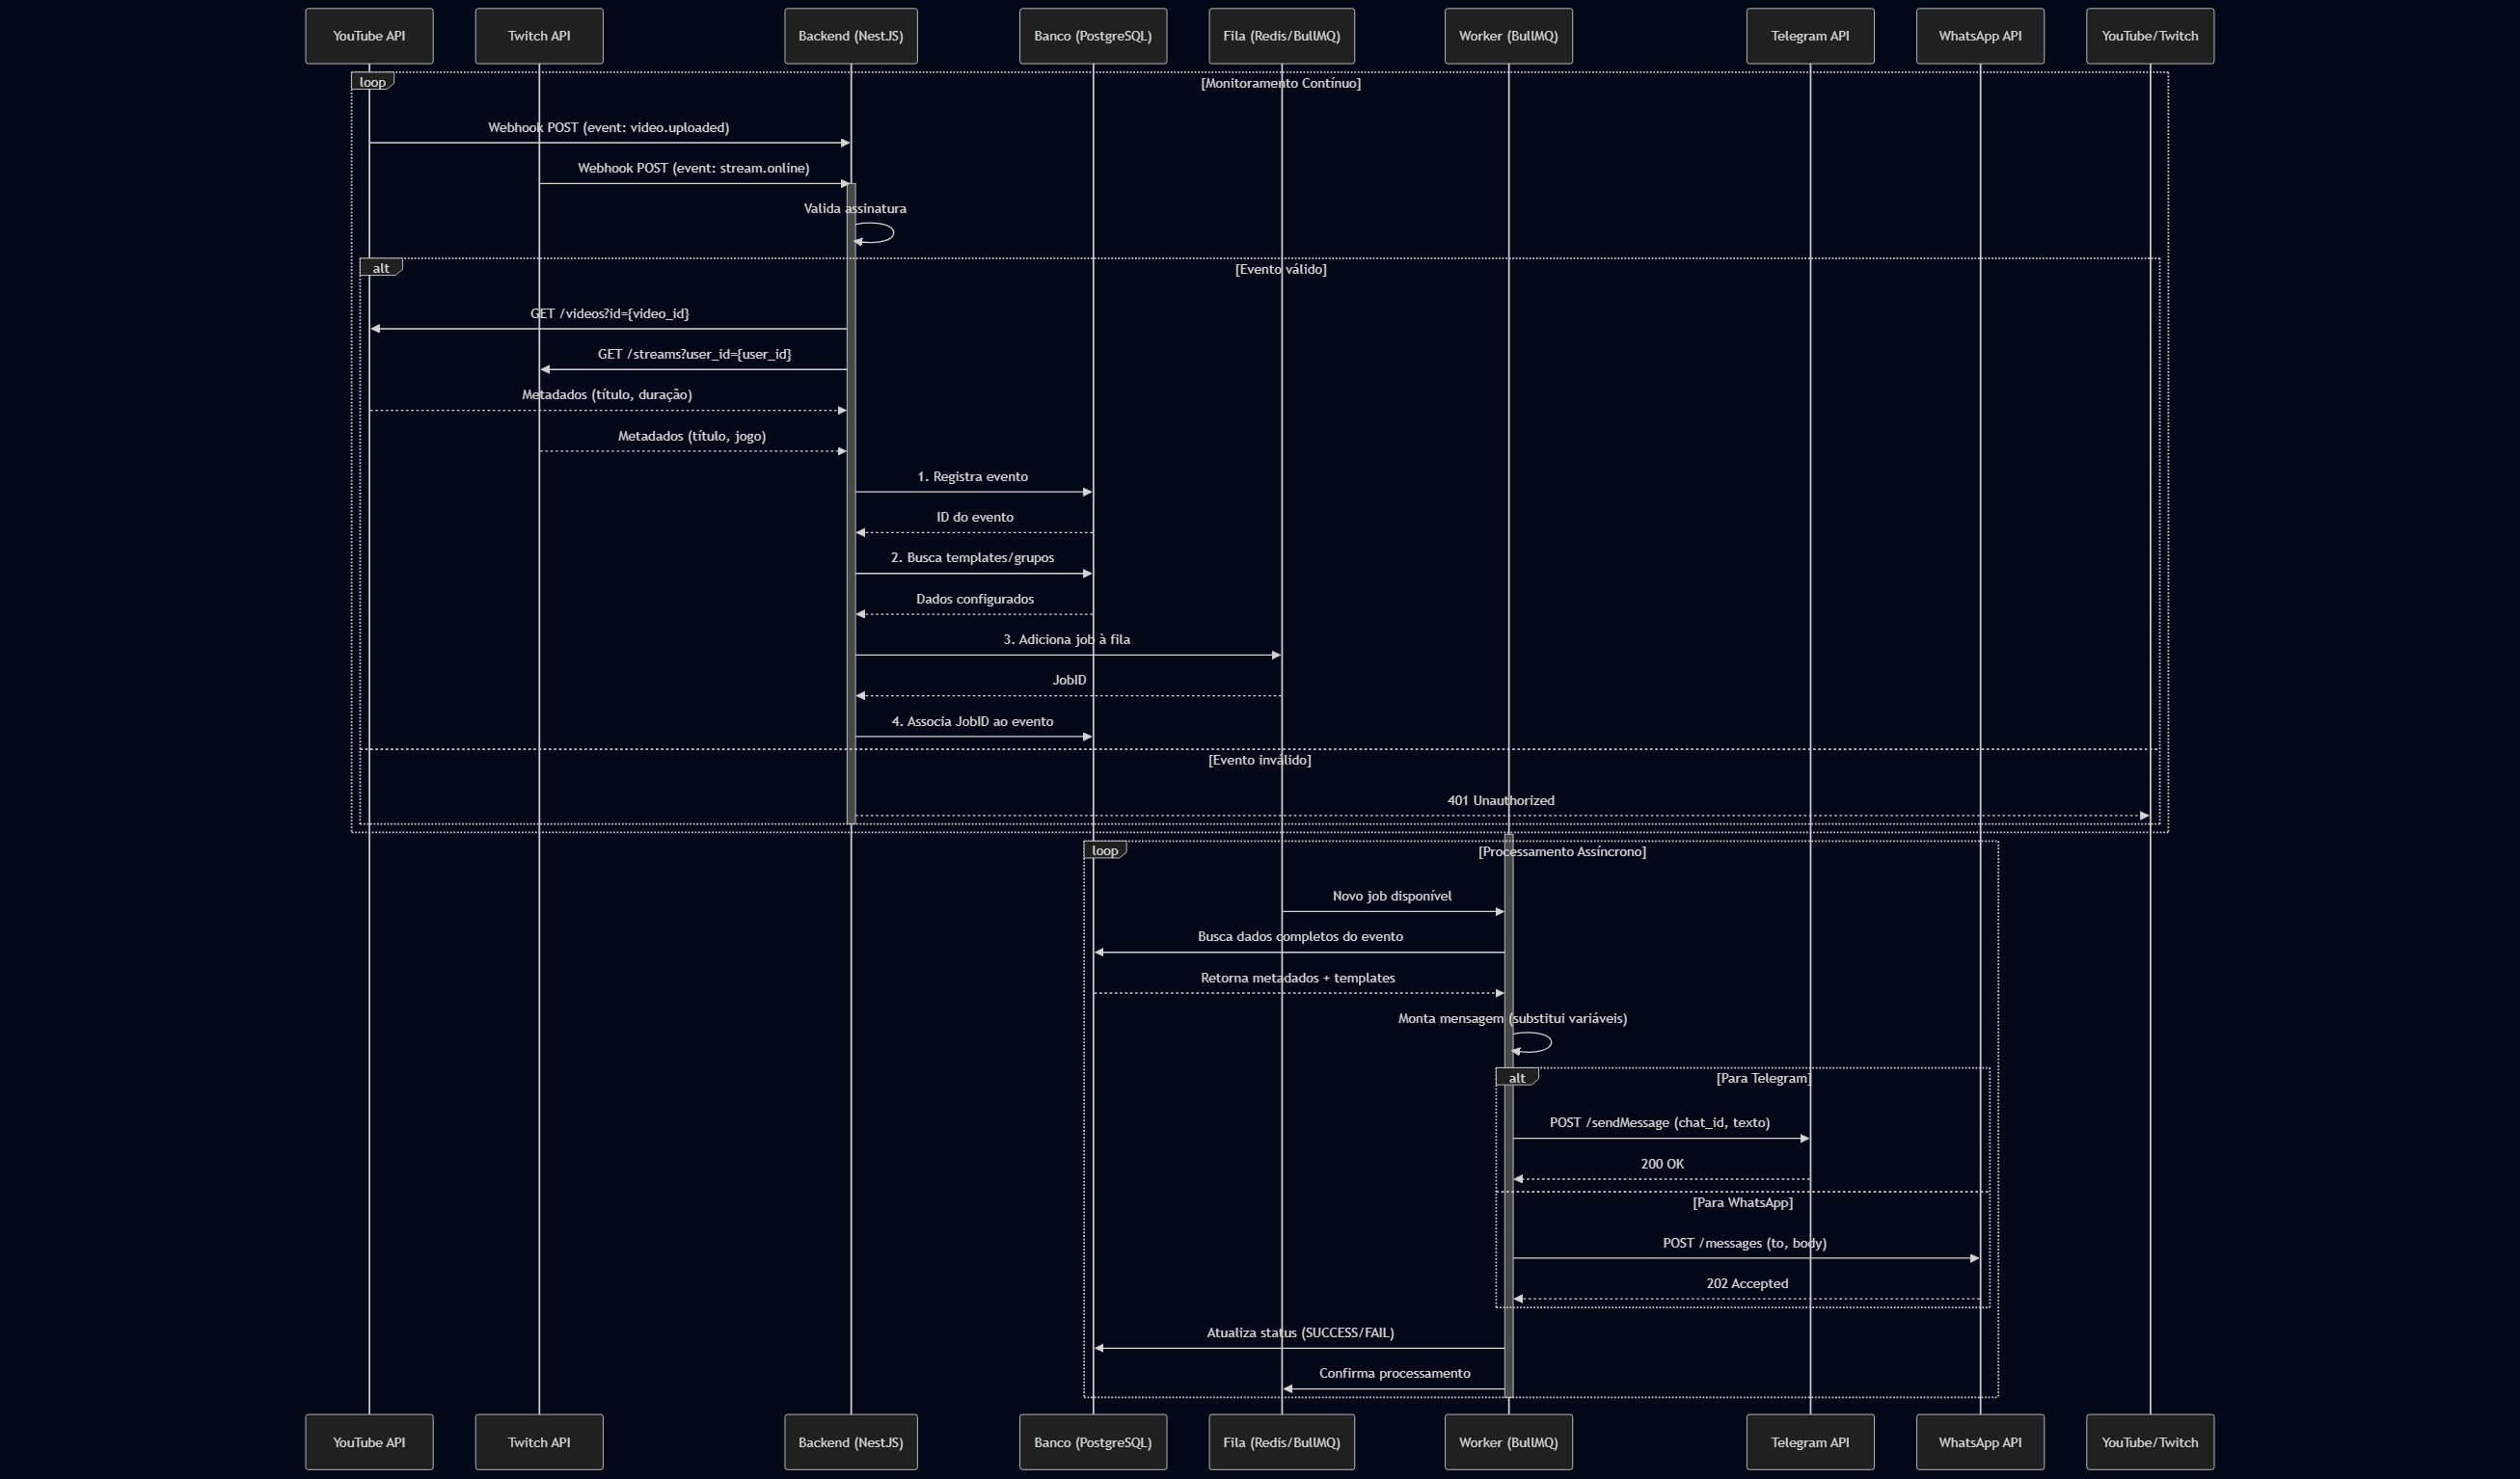
\includegraphics[width=0.9\textwidth]{img/Fluxo do Monitoramento de Eventos e Envio de Notificações.png}
            \label{fig:monitoramento}
        \end{figure}
    
        %##################  Imagem do Fluxo de Eventos e Envio de Notificações
        \begin{figure}[!ht]     
            \centering  
            \caption{
                Fluxo para Acessar o Histórico de Notificações Enviadas.\\ {\footnotesize\textbf{Fonte:} Autoria Própria.}
            }
            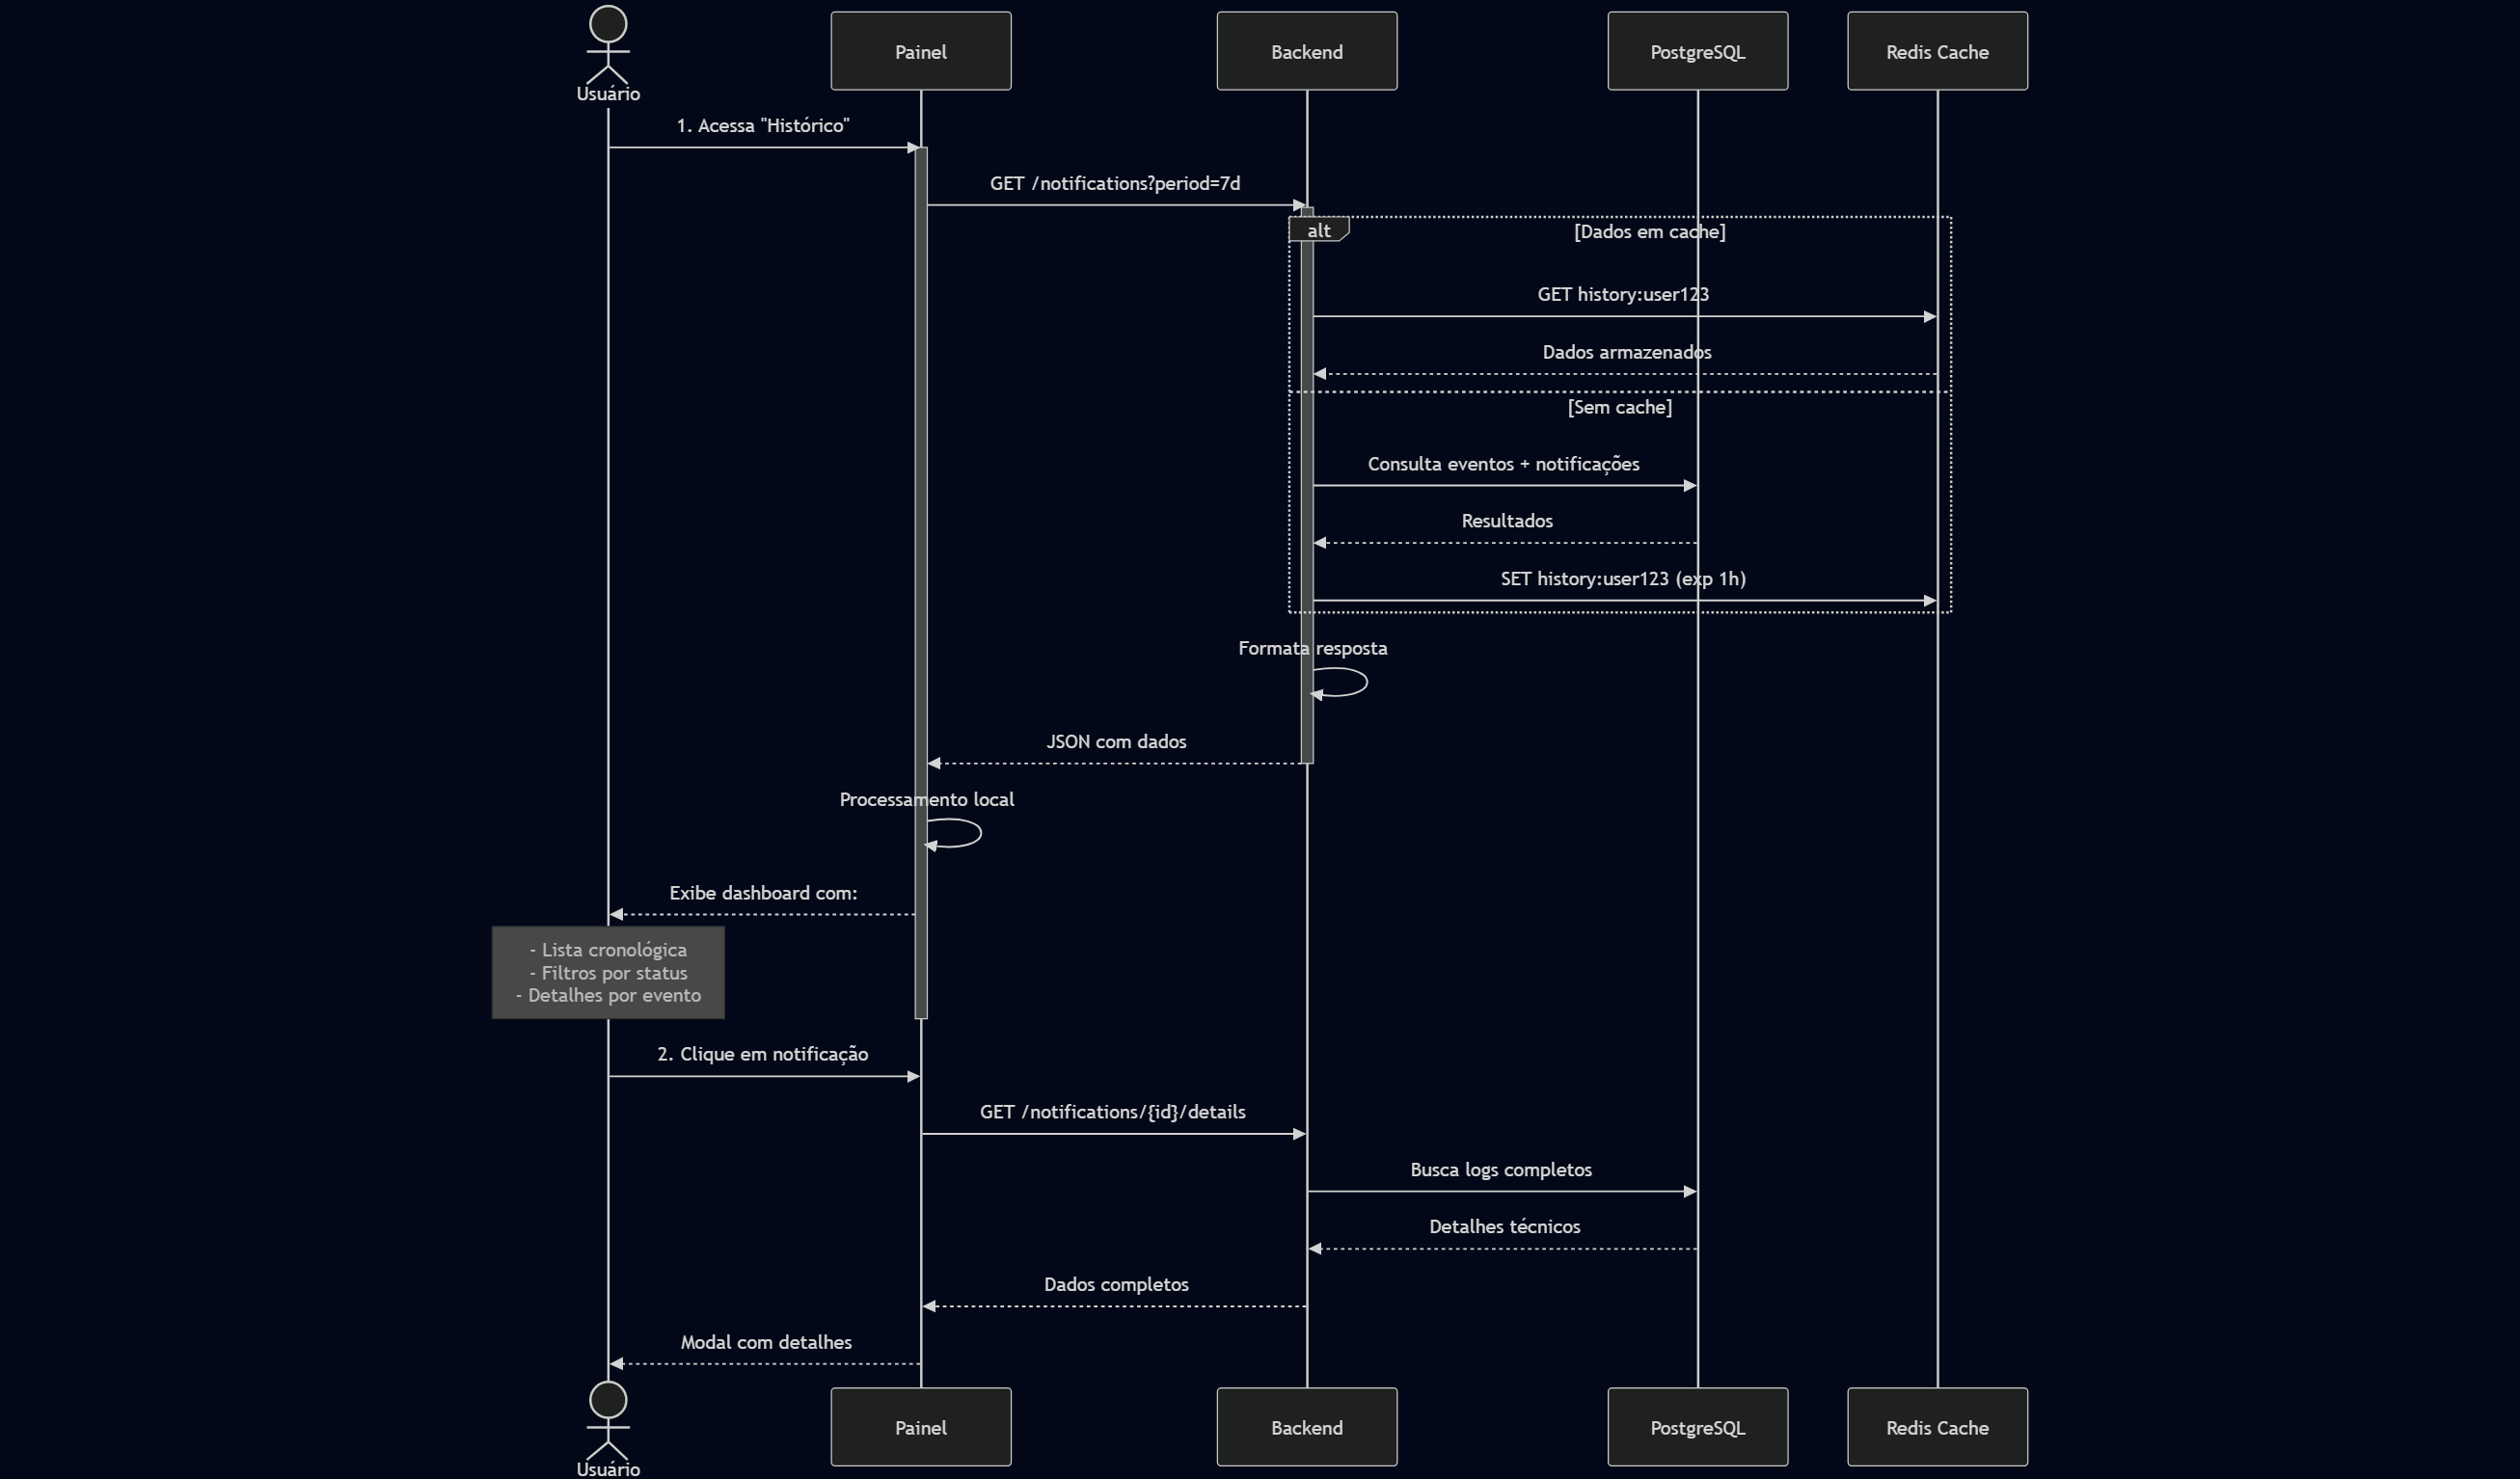
\includegraphics[width=0.9\textwidth]{img/Fluxo para Acessar o Histórico de Notificações Enviadas.png}
            \label{fig:historico}
        \end{figure}
        
        \item \textbf{Validação e testes}: 
            Após a conclusão da implementação, serão realizados testes funcionais para verificar o correto funcionamento do sistema, além de testes com usuários selecionados para avaliação da usabilidade.
        \par\vspace{0.25\baselineskip}
        
            \begin{itemize}
                \item \emph{Testes unitários}: 
                    Utilização do Jest para validar os módulos de integração, lógica de envio e demais componentes.  
                \par\vspace{0.25\baselineskip}
    
                \item \emph{Testes de integração}: 
                    Simulações de cenários reais (ex.: \textit{upload} de conteúdo, início de \textit{live}) utilizando Supertest e Jest.  
                \par\vspace{0.25\baselineskip}
    
                \item \emph{Testes de usabilidade}: 
                    Execução de testes com colegas ou usuários finais para avaliar a clareza do painel administrativo e a facilidade de configuração do sistema.  
                \par\vspace{0.5\baselineskip}
            \end{itemize}
        
        \item \textbf{Documentação e considerações finais}: 
            O projeto será documentado de forma completa, incluindo as decisões técnicas, limitações encontradas e sugestões para trabalhos futuros.
    \end{enumerate}
            
% Procedimentos Metodológicos/Metodologia-------------------------------------------------
% (máximo de 2 páginas)

% Na seção de procedimentos metodológicos ou metodologia (ver qual o nome mais adequado ao trabalho) deve ser descrito sucintamente o procedimentos metodológicos para a execução do projeto ressaltando como os objetivos serão alcançados. 

% Em geral, a seção descreve os procedimentos usados para resolver o problema atacado. Pode ser estruturada em tópicos, onde cada tópico representa um subproduto do objetivo geral.

% No caso de desenvolvimento de sistemas deve-se descrever a metodologia a ser utilizada, por exemplo Scrum, eXtreme Programming, RUP, etc. 

% Também pode ser descritos técnicas de desenvolvimento de software como por exemplo TDD, BDD, SPA,  etc.

% Coloque todos os materiais que serão utilizados. Exemplos: computadores, equipamentos de redes, licenças de software, etc. Também deverá ser colocado se os recursos estarão disponíveis. A universidade não comprará os recursos, portanto a responsabilidade de comprar algo será do aluno.

% (substitua este texto pelo de recursos necessários do trabalho)
    
%-----------------------------------------------------------------------------------------

\section{RESULTADOS ESPERADOS}
\label{sec:resultados}
% Recursos Necessários--------------------------------------------------------------------

Espera-se como principal resultado deste trabalho a entrega de uma aplicação Web funcional que automatize o envio de notificações personalizadas sobre novos vídeos e transmissões ao vivo em plataformas como YouTube e Twitch, direcionando essas mensagens para grupos no WhatsApp e Telegram. A aplicação deverá operar de forma segura e eficiente, utilizando autenticação via OAuth2 e processamento assíncrono com filas de tarefas.

O sistema também deverá incluir um painel administrativo simples e responsivo, que permita configurar canais, mensagens e destinos de forma intuitiva. Através de testes de integração, desempenho e usabilidade, espera-se validar a confiabilidade do sistema e a entrega correta das notificações. Além disso, o projeto proporcionará ao autor aprendizado prático em integração de APIs, desenvolvimento assíncrono e arquitetura de sistemas distribuídos, contribuindo para sua formação técnica e profissional.

%-----------------------------------------------------------------------------------------

\section{CRONOGRAMA}
\label{sec:planejamento}
% Planejamento do Trabalho----------------------------------------------------------------
% Esta seção não precisa ser editada, apenas edite o quadro 1 armazenada no diretório ".\dados\quadros"
O planejamento do trabalho a ser desenvolvido está detalhado no Quadro 1 – Cronograma de Atividades. Nele, estão listadas todas as etapas do projeto, organizadas conforme seus respectivos prazos de execução, garantindo uma estrutura clara para o cumprimento das atividades previstas em cada fase do Trabalho de Conclusão de Curso.

\begin{quadro}[H]
    %\centering
    \caption{Cronograma de Atividades.\label{qua:quadro1}}
    \begin{tabular}{|p{4.5cm}|p{0.7cm}|p{0.7cm}|p{0.7cm}|p{0.7cm}|p{0.7cm}|p{0.7cm}|p{0.7cm}|p{0.7cm}|p{0.7cm}|p{0.7cm}|}
        \hline
        \textbf{Atividades} & \textbf{Mar} & \textbf{Abr} & \textbf{Mai} & \textbf{Jun} & \textbf{Jul} & \textbf{Ago} & \textbf{Set} & \textbf{Out} & \textbf{Nov} & \textbf{Dez} \\
        \hline
        \small{1. Definição da proposta} & X &   &   &   &   &   &   &   &   &  \\
        \hline
        \small{2. Revisão bibliográfica e fundamentação do projeto} & X & X &   &   &   &   &   &   &   &  \\
        \hline
	\small{3. Redação do projeto de TCC} &   & X & X & X &   &   &   &   &   &  \\
        \hline
	\small{4. Defesa do projeto de TCC} &   &   &   & X &   &   &   &   &   &  \\
        \hline
	\small{5. Planejamento e especificação técnica detalhada} &   &   &   &   & X &   &   &   &   &  \\
        \hline
	\small{6. Desenvolvimento do sistema prático} &   &   &   &   & X & X & X & X &   &  \\
        \hline
        \small{7. Escrita da Monografia de TCC} &   &   &   &   &  & X & X & X & X &  \\
        \hline
        \small{8. Elaboração da apresentação final} &   &   &   &   &  &  &  &  & X &  \\
        \hline
	\small{9. Defesa final do TCC} &   &   &   &   &   &   &   &   &  & X\\
        \hline
    \end{tabular}
\end{quadro}

%-----------------------------------------------------------------------------------------

\section{CONSIDERAÇÕES FINAIS} % Escolher o nome mais adequado ao trabalho
\label{sec:conclusao}
% Conclusão/Considerações Finais----------------------------------------------------------
% (máximo de ½ página)
% Na seção de Conclusão ou Considerações Finais (ver qual o nome mais adequado ao trabalho) o acadêmico deve descrever:

% Como espera alcançar os objetivos propostos;

% Destacar as dificuldades encontradas e previstas;

% Fazer o fechamento do trabalho destacando sua importância.

Para alcançar os objetivos propostos, o projeto seguirá a metodologia detalhada no cronograma, dividida em etapas claras: pesquisa técnica das APIs (YouTube, Twitch, WhatsApp e Telegram), modelagem da arquitetura com NestJS e TypeScript, e implementação do sistema utilizando processamento assíncrono (BullMQ/Redis) para garantir escalabilidade. A validação ocorrerá via testes de integração (Supertest/Jest) e usabilidade, garantindo que as notificações sejam disparadas com confiabilidade e que o painel administrativo (Vue.js) seja intuitivo para configuração de canais e \textit{templates} de mensagem.

Quanto às dificuldades, destaca-se a complexidade na integração de APIs heterogêneas, especialmente o WhatsApp (via biblioteca não oficial), que impõe \textit{rate limits} e exige gestão rigorosa de \textit{tokens} OAuth2. Outro desafio é garantir a entrega oportuna de notificações em cenários de alta carga, exigindo otimização das filas (Redis) e tratamento de erros robusto. Além disso, a necessidade de autenticação em múltiplas plataformas pode gerar sobrecarga na manutenção do sistema.

Em síntese, este trabalho é relevante por oferecer uma solução unificada para um problema recorrente entre criadores de conteúdo: a divulgação manual e fragmentada de atividades em plataformas distintas. Ao automatizar notificações multicanal, o sistema promove eficiência operacional, maior engajamento de comunidades e acesso democratizado a ferramentas profissionais. Tecnicamente, contribui como estudo aplicado em arquitetura de sistemas distribuídos, integração de APIs e processamento assíncrono, servindo de base para futuras expansões (ex.: suporte a mais plataformas ou análises de métricas).

%-----------------------------------------------------------------------------------------